\documentclass[reprint, amsmath,amssymb, aps]{revtex4-2}

\usepackage{graphicx}
\usepackage{dcolumn}
\usepackage{bm}

\usepackage{setspace}

\usepackage{fancyhdr}
\setlength{\parindent}{0in}

% Page Formatting
\pagenumbering{arabic} %\pagenumbering{gobble}
\onehalfspacing %doublespacing
\pagestyle{fancy}
%\usepackage{pdfpages}

% Heading Formatting
\headheight 32pt

% Link Formatting
\usepackage{hyperref}
\hypersetup{
	colorlinks,
	allcolors=black
	%citecolor=black,
	%filecolor=black,
	%linkcolor=black,
	%urlcolor=black
}

\usepackage{mdframed}

% Code Formatting
\usepackage{listings}
% \lstset{
%         language=Python,
% 	basicstyle=\footnotesize,
% 	%numbers=left,
% 	stepnumber=1,
% 	showstringspaces=false,
% 	tabsize=1,
% 	breaklines=true,
% 	breakatwhitespace=false
% }

\lstset
{ %Formatting for code  
        language=Python,
	basicstyle=\footnotesize\ttfamily,
	numbers=left,
	%caption={},
	%title={},
	stepnumber=1,
	showstringspaces=false,
	tabsize=1,
	breaklines=true,
	breakatwhitespace=false,
	frame=lines,
	xleftmargin=2em,
	framexleftmargin=1.5em,
	%commentstyle=\color{commentsColor}\ttfamily,
  	%stringstyle=\color{stringColor}\ttfamily,
	%keywordstyle=\color{keywordsColor}\bfseries,
}

% Figures & Drawings
%\usepackage{graphicx, caption}
%\usepackage{animate}
\usepackage{tikz}
\usepackage{float}
\usepackage{pict2e}
\usepackage{subcaption}

% Physics
\usepackage{physics}

% Mathematics
\usepackage{amsmath}
\usepackage{amssymb}
\usepackage{amsthm}
\usepackage{mathtools}
\usepackage{mathrsfs}
\usepackage{upgreek} % More Greek letters

% I don't really know what this is but I don't want to break shit
\usepackage{aliascnt}
\newaliascnt{eqfloat}{equation}
\newfloat{eqfloat}{h}{eqflts}
\floatname{eqfloat}{Equation}
\newcommand*{\ORGeqfloat}{}
\let\ORGeqfloat\eqfloat
\def\eqfloat{%
	\let\ORIGINALcaption\caption
	\def\caption{%
		\addtocounter{equation}{-1}%
		\ORIGINALcaption
	}%
	\ORGeqfloat
}
%}

% Bibliography (Citations) Formatting

%\usepackage{cite}
%\usepackage{caption}

%\usepackage[backend=bibtex,style=verbose-trad2]{biblatex}
%works really really well, but no MLA format
%\bibliographystyle{apsrev4-1}
%\usepackage{biblatex}
%\usepackage[backend=biber]{biblatex}
%\usepackage[backend=biber,style=mla]{biblatex} %Doesn't print all sources for some reason

\usepackage{pgfplots}

% Tikz Packages
\usepackage{circuitikz}


\tikzset{>=latex} % for LaTeX arrow head
\colorlet{myred}{red!85!black}
\colorlet{mydarkred}{red!55!black}
\colorlet{mylightred}{red!85!black!12}
\colorlet{myfieldred}{mydarkred!5} % for S' background
\colorlet{myredhighlight}{myred!20} % highlights simultaneity in ladder paradox
\colorlet{myblue}{blue!80!black}
\colorlet{mydarkblue}{blue!50!black}
\colorlet{mylightblue}{blue!50!black!30}
\colorlet{mylightblue2}{myblue!10}
\colorlet{mygreen}{green!80!black}
\colorlet{mypurple}{blue!40!red!80!black}
\colorlet{mydarkgreen}{green!50!black}
\colorlet{mydarkpurple}{blue!40!red!50!black}
\colorlet{myorange}{orange!40!yellow!95!black}
\colorlet{mydarkorange}{orange!40!yellow!85!black}
\colorlet{mybrown}{brown!20!orange!90!black}
\colorlet{mydarkbrown}{brown!20!orange!55!black}
\colorlet{mypurplehighlight}{mydarkpurple!20} % highlights simultaneity in ladder paradox
\tikzstyle{world line}=[myblue!40,line width=0.3]
\tikzstyle{world line t}=[mypurple!50!myblue!40,line width=0.3]
\tikzstyle{world line'}=[mydarkred!40,line width=0.3]
\tikzstyle{mysmallarr}=[-{Latex[length=3,width=2]},thin]
\tikzstyle{mydashed}=[dash pattern=on 3 off 3]
\tikzstyle{rod}=[mydarkbrown,draw=mydarkbrown,double=mybrown,double distance=2pt,
                 line width=0.2,line cap=round,shorten >=1pt,shorten <=1pt]
%\tikzstyle{rod'}=[rod,draw=mydarkbrown!80!red!85,double=mybrown!80!red!85]
\tikzstyle{vector}=[->,line width=1,line cap=round]
\tikzstyle{vector'}=[vector,shorten >=1.2]
\tikzstyle{particle}=[mygreen,line width=0.9]
\tikzstyle{photon}=[-{Latex[length=5,width=4]},myorange,line width=0.8,decorate,
                    decoration={snake,amplitude=1.0,segment length=5,post length=5}]

\def\tick#1#2{\draw[thick] (#1) ++ (#2:0.06) --++ (#2-180:0.12)}
\def\tickp#1#2{\draw[thick,mydarkred] (#1) ++ (#2:0.06) --++ (#2-180:0.12)}
\def\Nsamples{100} % number samples in plot
\usetikzlibrary{quantikz2}

% Custom Symbols 
%{
\newcommand\halmos{\rule{.36em}{2ex}} % Custom QED Symbol
\def\contradict{\tikz[baseline, x=0.22em, y=0.22em, line width=0.032em]\draw (0,2.83)--(2.83,0) (0.71,3.54)--(3.54,0.71) (0,0.71)--(2.83,3.54) (0.71,0)--(3.54,2.83);}
\renewcommand{\qedsymbol}{\halmos}
\renewenvironment{proof}{{\bfseries \textit{Proof} \\}}{\qedsymbol}

\makeatletter
\newcommand{\crossout}[1]{% Crosses out symbol
	\begingroup
	\settowidth{\dimen@}{#1}%
	\setlength{\unitlength}{0.05\dimen@}%
	\settoheight{\dimen@}{#1}%
	\count@=\dimen@
	\divide\count@ by \unitlength
	\begin{picture}(0,0)
		\put(0,0){\line(20,\count@){20}}
		\put(0,\count@){\line(20,-\count@){20}}
	\end{picture}%
	#1%
	\endgroup
}
%}

% Mathematics (General)
\newtheorem{theorem}{Theorem}[section]
\newtheorem{corollary}{Corollary}[theorem]
\newtheorem{lemma}[theorem]{Lemma}

\newtheoremstyle{named}{}{}{\itshape}{}{\bfseries}{.}{.5em}{\thmnote{#3}#1}
\theoremstyle{named}
\newtheorem*{namedtheorem}{Theorem}

\newcommand{\lemref}[1]{\textit{Lemma \ref{#1}}}
\newcommand{\thmref}[1]{\textbf{Theorem \ref{#1}}}
\newcommand{\colref}[1]{\textit{Corollary \ref{#1}}}

% Physics (Quantum Mechanics)
%\newcommand{\norm}[#1]{\lVert {#1} \rVert}
%\newcommand{\ket}[1]{\vert{#1}\rangle}
%\newcommand{\bra}[1]{\langle{#1}\vert}
%\newcommand{\braket}[2]{\langle {#1} \vert {#2} \rangle}
\newcommand{\expectation}[1]{\langle{#1}\rangle}

% Physics (Electrodynamics)
\newcommand{\del}{\overline{\nabla}}
\usetikzlibrary{arrows}
%Script r (scalar)
\newcommand{\rc}{%
\resizebox{!}{1.25ex}{%
    \begin{tikzpicture}[>=round cap]
        \clip (0.09em,-0.05ex) rectangle (0.61em,0.81ex);
        \draw [line width=.11ex, <->, rounded corners=0.13ex] (0.1em,0.1ex) .. controls (0.24em,0.4ex) .. (0.35em,0.8ex) .. controls (0.29em,0.725ex) .. (0.25em,0.6ex) .. controls (0.7em,0.8ex) and (0.08em,-0.4ex) .. (0.55em,0.25ex);
    \end{tikzpicture}%
}%
}

%Script r (vector)
\newcommand{\brc}{%
\resizebox{!}{1.3ex}{%
    \begin{tikzpicture}[>=round cap]
        \clip (0.085em,-0.1ex) rectangle (0.61em,0.875ex);
        \draw [line width=.2ex, <->, rounded corners=0.13ex] (0.1em,0.1ex) .. controls (0.24em,0.4ex) .. (0.35em,0.8ex) .. controls (0.29em,0.725ex) .. (0.25em,0.6ex) .. controls (0.7em,0.8ex) and (0.08em,-0.4ex) .. (0.55em,0.25ex);
    \end{tikzpicture}%
}%
}

%Script r with a hat (unit vector)
\newcommand{\hrc}{\hat{\brc}}


% Document (General)
\newcommand{\figref}[1]{Fig. \ref{#1}}
\newcommand{\source}[1]{\caption*{Source: {#1}} }
\newcommand{\graphdata}[1]{\caption*{Fit Parameters: {#1}}}
%\newenvironment{\drawpicture}[1][]{\resizebox{<horizontal size>}{<vertical size>}{ \begin{tikzpicture}}{\end{tikzpicture}}}
\newcommand{\Q}{\mathbb{Q}}



% ========================================= %
% Change for each document [!!!]
\newcommand\course{PHY365}	% Course Code [!!!]
\newcommand\doctitle{Final Exam Revision} % Report Title [!!!]
\newcommand\firstauthorname{Aditya K. Rao 1008307761}
\newcommand\taname{D.F.V. James} % TA Name [!!!]
\newcommand{\location}{\texttt{April 25, 2024}} % Location [!!!]
% ========================================= %
 
%\pagenumbering{gobble}
\usepackage{listings}

\renewcommand\lstlistingname{Code Reference}
\renewcommand\lstlistlistingname{Code Reference}
\usepackage{tikz}
\usetikzlibrary{patterns}


\begin{document}

\title{\course \ \doctitle}
\author{\firstauthorname}
\affiliation{University of Toronto}

%\collaboration{Advisor}

\date{April 25, 2024} %Put in date of submission [!!!]

\preprint{APS/123-QED}

%\title{Manuscript Title:\\with Forced Linebreak}% Force line breaks with \\
\thanks{\textbf{Date:} \location}%

% \begin{abstract}
%     Compilation of all my lecture notes and solutions for the course PHY365 taught by Professor DFV James at the University of Toronto during the 2024 Winter Semester. PHY365 is the University of Toronto's undergraduate introduction to Quantum Information course and covers a wide range of content. 
%     \begin{description}
%         \item[Accuracy]  I cannot guarantee the accuracy of these notes nor the accuracy of the information they contain with absolute certainty though they are likely accurate.
%         \item[Copyright] The notes written here are my own and my authorization is required before distribution to any other party. Moreover, the information contained in this document is from the course taught by Professor James and thus, he should be consulted prior to distributing these notes. Specifically, problem set questions are contained within this document which are the copyright of Professor James.
%     \end{description}
% \end{abstract}

% \begin{abstract}
% \end{abstract}

    \maketitle
    \tableofcontents
    %\thispagestyle{empty}
    \clearpage
    %\pagenumbering{arabic}
    %So the heading doesn't show up on table of contents page
	%\lhead{\yourname\ \vspace{0.1cm} \\ \course}
	\lhead{\firstauthorname\vspace{0.1cm}}
        \chead{\textbf{\course} \\ \doctitle}
        \rhead{\textbf{Prof:} \taname \\ \textbf{Date:} \location}

    \section{Definitions} \label{sec:intro} 
        \subsection{Dirac Notation of Qubits in this Course}
            

        \subsection{Reading Circuit Diagrams}    
            \begin{figure}[H]
                \centering
                \begin{quantikz}
                    \lstick{$\ket{\varphi_1}$} & \ctrl{1} & \rstick{$\ket{\psi}_1$} \\
                    \lstick{$\ket{\varphi_0}$} & \targ{1} &  \rstick{$\ket{\psi}_0$}
                \end{quantikz}
                \caption{Controlled not gate, the control is the black dot and the target is the $\oplus$. The $\oplus = \hat{X}$ by convention. The output is no longer necessarily a pure state.}
                \label{fig:cnot-gate}
            \end{figure}

        \subsubsection{Unitary \& Pauli Gates}
            \begin{figure}[H]
                \centering
                \begin{quantikz}
                   \lstick{$\ket{\varphi}$} & \gate{U} &  \rstick{$\hat{U}\ket{\varphi}$}
                \end{quantikz}
                \caption{Local unitary (substitute $U$ for $X$, $Y$, $Z$, or $H$ for the desired unitary)}
                \label{fig:unitary-gate}
            \end{figure}
            
            \paragraph{Generic Unitary Gate}
                % \begin{align*}
                %     \hat{U} &= \begin{bmatrix}a & b \\b^{*} & a\end{bmatrix} \begin{cases}\hat{X}\ket{0} = \ket{1} \\ \hat{X}\ket{1} = \ket{0}\end{cases}
                % \end{align*}
            
            \paragraph{Pauli-X Gate}
                \begin{align*}
                    \hat{X} &= \begin{bmatrix}0 & 1 \\1 & 0\end{bmatrix} \begin{cases}\hat{X}\ket{0} = \ket{1} \\ \hat{X}\ket{1} = \ket{0}\end{cases}
                \end{align*}
            \paragraph{Pauli-Z Gate}
                \begin{align*}
                    \hat{Z} &= \begin{bmatrix}1 & 0 \\0 & -1\end{bmatrix}\begin{cases}\hat{Z}\ket{0} = \ket{0} \\ \hat{Z}\ket{1} = -\ket{1}\end{cases}
                \end{align*}
    
            \paragraph{Pauli-Y Gate}
                \begin{align*}
                    \hat{Y} &= \begin{bmatrix}0 & -i \\i & 0\end{bmatrix}\begin{cases}\hat{Y}\ket{0} = i\ket{1} \\ \hat{Y}\ket{1} = \ket{0}\end{cases}
                \end{align*}
    
            \paragraph{Hadamard Gate}
                \begin{align*}
                    \hat{H} &= \frac{1}{\sqrt{2}}\begin{bmatrix}1 & 1 \\1 & -1\end{bmatrix}\begin{cases}\hat{H}\ket{0} =\frac{\ket{0}+\ket{1}}{\sqrt{2}} \\ \hat{H}\ket{1} = \frac{\ket{0}-\ket{1}}{\sqrt{2}}\end{cases}
                \end{align*}
    
        \subsubsection{Measurement Operations} \label{sec:def-q-measurement}
            \begin{figure}[H]
                \centering
                \begin{quantikz}
                    \lstick{$\ket{\varphi}$} & \meter{} & \setwiretype{c}\rstick{$\{\ket{0},\ket{1}\}$}
                \end{quantikz}
                \caption{Measurement operation. After the measurement the state collapses into a classical bit represented by the double wires.}
                \label{fig:unitary-gate}
            \end{figure}
            
            \begin{equation*}
                \texttt{MEASUREMENT} = \ket{0}\bra{0} + \ket{1}\bra{1}
            \end{equation*}
            \begin{equation} \label{eqn:cnot-dirac}
                \texttt{CNOT} = \ket{0}\bra{0}\otimes\hat{I} + \ket{1}\bra{1}\otimes\hat{X} 
                \begin{cases}
                \texttt{CNOT}(\ket{00}) = \ket{00} \\
                \texttt{CNOT}(\ket{10}) = \ket{11} \\
                \texttt{CNOT}(\ket{01}) = \ket{01} \\
                \texttt{CNOT}(\ket{11}) = \ket{10}
                \end{cases}
            \end{equation}

        \subsubsection{Controlled Unitaries}

            \begin{figure}[H]
                \centering
                \begin{quantikz}
                    \lstick{$\ket{\varphi_1}$} & \ctrl{1} & \rstick{$\ket{\psi}_1$} \\
                    \lstick{$\ket{\varphi_0}$} & \targ{1} &  \rstick{$\ket{\psi}_0$}
                \end{quantikz}
                \caption{Controlled not gate, the control is the black dot and the target is the $\oplus$. The $\oplus = \hat{X}$ by convention. The output is no longer necessarily a pure state.}
                \label{fig:unitary-gate}
            \end{figure}

            \begin{equation} \label{eqn:cnot-dirac}
                \texttt{C}\hat{U} = \ket{0}\bra{0}\otimes\hat{I} + \ket{1}\bra{1}\otimes\hat{U} 
                \begin{cases}
                \texttt{C}\hat{U}(\ket{00}) = \ket{00} \\
                \texttt{C}\hat{U}(\ket{10}) = \ket{01} \\
                \texttt{C}\hat{U}(\ket{01}) = \ket{1}\hat{U}\ket{0} \\
                \texttt{C}\hat{U}(\ket{11}) = \ket{1}\hat{U}\ket{1}
                \end{cases}
            \end{equation}

        \subsubsection{Example: Quantum Teleportation}

            \begin{figure}
                \centering
                \begin{quantikz}
                \lstick{$\ket{\varphi}$} \slice{$\ket{\psi_{0}}$} & &\slice{$\ket{\psi_{1}}$} & \ctrl{1} & \gate{H}\slice{$\ket{\psi_{2}}$} & \meter{} & \setwiretype{c} & \ctrl[vertical wire=c]{0} & & \\
                \lstick{$\ket{0}$} & \gate{H} & \ctrl{1} & \targ{1} & & \meter{}&\ctrl{0} \setwiretype{c} & & &  \\
                \lstick{$\ket{0}$} & & \targ{1} & & & &\gate{X}\wire[u][1]{c} &\gate{Z}\wire[u][2]{c} & & \rstick{$\ket{\varphi}$}
                \end{quantikz}
                \caption{Quantum teleportation circuit as described (with modification) in Neilson \& Chuang \cite{nielsen_chuang_2010}. The first Hadamard ($\hat{H}$) and CNOT gates describes the creation of a bell state.}
                \label{fig:teleport}
            \end{figure}
            In order to more explicitly see the state teleportation, the mathematics will explicitly be shown at each key step. Each qubit can generally be referred to as $\Q_n$ where $n$ is the index of the qubit. Qubits are indexed from \textbf{bottom to top} in circuit diagrams and \textbf{right to left} in Dirac notation.
            
            For clarity the state to be teleported is $\ket{\varphi}$ whereas the global state of the system is denoted with $\ket{\psi_{t}}$ where $t$ is the global state after some number of time steps. Generally, $\ket{\varphi}$ can be represented in \eqref{eqn:general-initial-state}.
        
            \begin{equation} \label{eqn:general-initial-state}
                \ket{\varphi} = \alpha\ket{0} + \beta\ket{1}
            \end{equation}
            Where $\ket{0}$ and $\ket{1}$ are the basis of the \texttt{spin-1/2} system. the initial global state $\ket{\psi_0}$ can hence be represented in \eqref{eqn:global-state-0}. Note that the subscripts represent the qubit index. 
            \begin{align}
                \ket{\psi_0} &= \ket{\varphi}_2\ket{0}_1\ket{0}_0 \ \text{(Qubit index explicitly noted)} \\
                &= \alpha\ket{0}_{2}\ket{0}_{1}\ket{0}_{0} + \beta\ket{1}_{2}\ket{0}_{1}\ket{0}_{0} \\
                &= \alpha\ket{000} + \beta\ket{100} \label{eqn:global-state-0}
            \end{align}
            Now induce a bell state \footnote{Also known as an EPR Pair or an entangled state} using a Hadamard gate and a \textit{CNOT} gate (Controlled $X$ gate). This can be seen in \eqref{eqn:global-state-1}
            \begin{align}
                \ket{\psi_1} =& \texttt{CNOT}\ \hat{H}\{\alpha\ket{000} + \beta\ket{100}\} \\
                \begin{split}
                =& \texttt{CNOT}\{\frac{\alpha}{\sqrt{2}}\ket{0}(\ket{0}+\ket{1})\ket{0} \\ &+\frac{\beta}{\sqrt{2}}\ket{1}(\ket{0}+\ket{1})\ket{0}\} 
                \end{split}\\
                =& \frac{1}{\sqrt{2}}\texttt{CNOT}\{\alpha\ket{000} + \alpha\ket{010} + \beta\ket{100} + \beta\ket{110}\} \\
                \begin{split}
                =& \frac{1}{\sqrt{2}}(\ket{0}\bra{0}\otimes\hat{I}+\ket{1}\bra{1}\otimes\hat{X})\{\alpha\ket{000} + \alpha\ket{010} \\
                &+ \beta\ket{100} + \beta\ket{110}\} \label{eqn:global-state-1-intermediate} \\
                \end{split}\\
                =& \frac{1}{\sqrt{2}}\{\alpha\ket{000} + \alpha\ket{011} + \beta\ket{100} + \beta\ket{111}\} \label{eqn:global-state-1}
            \end{align}
            Once a bell state has been prepared, $\Q_0$ can be separated an arbitrary distance from $\Q_1$ and $\Q_2$. In order to actually teleport the state of $\Q_2 = \ket{\varphi}$ to $\Q_0$, an additional interaction must be performed through local interactions on $\Q_2$ and $\Q_1$. This is $\ket{\psi_2}$ and is calculated in \eqref{eqn:global-state-2}.
            \begin{align}
                \ket{\psi_2} =& \frac{1}{\sqrt{2}}\hat{H}\ \texttt{CNOT}\{\alpha\ket{000} + \alpha\ket{011} \beta\ket{100} + \beta\ket{111}\} \\
                =& \frac{1}{\sqrt{2}}\hat{H} \{\alpha\ket{000} + \alpha\ket{011} \beta\ket{110} + \beta\ket{101}\} \\
                \begin{split}
                =& \frac{1}{2} \{\alpha(\ket{0}+\ket{1})\ket{00} + \alpha(\ket{0}+\ket{1})\ket{11} \\
                &+ \beta(\ket{0}-\ket{1})\ket{10} + \beta(\ket{0}-\ket{1})\ket{01}\} \\
                \end{split}\\
                \begin{split}
                =& \frac{1}{2} \{\alpha\ket{000} + \alpha\ket{100} + \alpha\ket{011}+\alpha\ket{111} \\
                &+ \beta\ket{010}-\beta\ket{110} + \beta\ket{001} -\beta\ket{101}\} \label{eqn:global-state-2}
                \end{split}
            \end{align}
            At this point the teleportation is completed, this can be explicitly be seen through simple rearrangement in \eqref{eqn:global-state-2-re} rearranged. The final controlled measurements are meant as a `correction' to flip and change signs to exactly obtain $\ket{\varphi}$.
        
            \begin{align}
                \begin{split}
                \ket{\psi_2} =& \frac{1}{2} \{\ket{00}(\alpha\ket{0} + \beta\ket{1}) + \ket{10}(\alpha\ket{0} - \beta\ket{1}) \\
                &+ \ket{01}(\alpha\ket{1}+\beta\ket{0})+\ket{11}(\alpha\ket{1}-\beta\ket{0})\} \\
                \end{split}\\
                \begin{split}
                =& \frac{1}{2}\{\ket{00}(\ket{\varphi}) + \ket{10}(\hat{Z}\ket{\varphi}) \\
                &+ \ket{01}(\hat{X}\ket{\varphi})+\ket{11}(\hat{X}\hat{Z}\ket{\varphi})\} \label{eqn:global-state-2-re} \\
                \end{split}\\
                \begin{split}
                =& \frac{1}{2}\{\ket{0}_2\ket{0}_1(\ket{\varphi}_0) + \ket{1}_2\ket{0}_1(\hat{Z}\ket{\varphi}_0) \\
                &+ \ket{0}_2\ket{1}_1(\hat{X}\ket{\varphi}_0)+\ket{1}_2\ket{1}_1(\hat{X}\hat{Z}\ket{\varphi}_0)\}  \\
                &\text{(Qubit indices explicitly noted)} \\
                \end{split}
            \end{align}
        
    \section{Concepts}
        \subsection{Fundamentals}
            \subsubsection{Single Qubit Gates}

            \subsubsection{Two Qubit Gates}
                One can try applying unitaries to create entanglement but this won't work. this is because \textbf{localized operations} don't change entanglement. Instead one has two use a \textit{two qubit gate}. 
                

            \subsection{Time Evolution}
                
            \subsubsection{Bell's Inequalities}
                Consider a state
                \begin{equation*}
                    \ket{\beta_0} = \frac{1}{\sqrt{2}} (\ket{00}+\ket{11}) = \ket{\Phi_{+}}
                \end{equation*}

                Notice that if you measure $\Q_1$, \textbf{instantaneously}, $\Q_2$ collapses on the same state as the outcome of the measurement of $\Q_1$.  The idea of instantaneous influence may violate the principle of special relativity (\textit{Einstein-Podolsky-Rosen Paradox} \cite{epr}).

                States such as these are known as \textbf{Bell States} and are \textbf{maximally entangled}. There are 4-bell states

                \begin{align*}
                    \ket{\beta_0} = \ket{\Phi_{+}} &= \frac{1}{\sqrt{2}}(\ket{00} + \ket{11}) \\
                    \ket{\beta_1} = \ket{\Psi_{-}} &= \frac{i}{\sqrt{2}}(\ket{01} + \ket{10}) = I\otimes\sigma_1 \ket{\beta_0}\\
                    \ket{\beta_2}  = \ket{\Psi_{+}} &= \frac{-1}{\sqrt{2}}(\ket{01} - \ket{10}) = I\otimes\sigma_2 \ket{\beta_0} \\
                    \ket{\beta_3} =  = \ket{\Phi_{-}} &= \frac{i}{\sqrt{2}}(\ket{00} - \ket{11}) = I\otimes\sigma_3 \ket{\beta_0}
                \end{align*}

                Together these form an orthonormal basis known as the \textbf{bell basis} or the \textbf{singlet basis} (or some other permutation). An example state in this basis can be seen below
                \begin{align*}
                \ket{\psi} &= A\ket{\beta_0} + B \ket{\beta_1} + C\ket{\beta_2} + D\ket{\beta_0}
                 \\
                &= \frac{A+Di}{\sqrt{2}}\ket{00} + \frac{iB - C}{\sqrt{2}}\ket{10} + \cdots
                \end{align*}

                Now we can see $\alpha = \frac{A+Di}{\sqrt{2}}$ and so on. Using \eqref{eqn:concurence}, one can obtain the concurrence as:

                \begin{align*}
                    C &= 2|\alpha\delta - \gamma\beta| \\
                      &= 2|\frac{1}{2}(A+iD)(A-iD) - \frac{1}{2}(iB-C)(iB+C)| \\
                      &= |A^2 + B^2 + C^2 + D^2| 
                \end{align*}

                \begin{theorem} \textbf{The Fundamental Theorem of Entanglement}
                    \begin{align*}
                        (I\otimes U)\ket{\beta_2} =& -\frac{1}{\sqrt{2}} (\ket{0}\otimes(b\ket{0}+a^*\ket{1})\\
                        &-\ket{1}\otimes(a\ket{0}-b^*\ket{1}))\\
                        =& -(U^\dagger\otimes I )\ket{\beta_2} \\
                        \therefore (U\otimes U)\ket{\beta_2} =& -\ket{\beta_2}
                    \end{align*}

                    A unitary applied to $\Q_0$ in a maximally entangled (in singlet basis) pair is equivalent to applying a related \footnote{vague, but it involves either the same and negative or applying a few Pauli operators and other unitaries} unitary to $\Q_1$ of the pair
                    
                \end{theorem}

                \subsubsection{Hidden variables and why they don't work}
                    Recall \S\ref{sec:def-q-measurement}, however, instead of 0 and 1, lets measure -1 and 1 to create this definition we must redefine an operator as such:
                    \begin{align*}
                    \hat{a} \ \text{(operator)} &= \vec{a}\cdot\hat{\sigma} \\
                    &= a_x\hat{X} +a_y\hat{Y}+a_z\hat{Z} \\
                    &= \begin{bmatrix}a_z & a_x - i a_y \\ a_x-ia_y & -a_z\end{bmatrix}
                    \end{align*}
    
                    where $\vec{a}$ is a \textbf{vector}, $\hat{\sigma}$ are the Pauli operators, and $\hat{a}$ is an operator. This gives us the eigenvalues $-1$ and $1$ as desired for these measurements. Define the average of $\vec{a}$ as $\overline{a}$ to obtain the following:
    
                    \begin{align*}
                    \overline{a} &= \int a(\lambda)p(\lambda) \ d\lambda \\
                    &= \braket{\hat{a}} = \text{Quantum Prediction}
                    \end{align*}

                    Let us consider some hidden-variable theory. For the hidden variable theory to be true, there must be something about it which avoids Bell's inequalities.
    
                    One can ``test'' this with Bell's inequalities as follows. Consider a circuit as in figure \ref{fig:measurement-operations-bell}.
    
                    \begin{figure}
                        \centering
                        \begin{quantikz}
                            \lstick{$\ket{0}$} & \gate{H} & \ctrl{1} & \gate{Y} & \gate{U} & \meter{} & \setwiretype{c} \\
                            \lstick{$\ket{0}$} & & \gate{U} &&& \meter{} & \setwiretype{c}
                        \end{quantikz}
                        \caption{Measurement Operations and Bell's inequalities}
                        \label{fig:measurement-operations-bell}
                    \end{figure}

                    Where $\Q_0$ U is $\frac{\hat{a}}{\hat{b}}$ and $\Q_1$ U is $\frac{\hat{c}}{\hat{d}}$. Using the idea of a hidden variable, one can obtain the following

                    \begin{equation*}
                        \mathscr{S} = \{a(\lambda) + b(\lambda)\}c(\lambda) + {a(\lambda)-b(\lambda)}d(\lambda)
                    \end{equation*}

                    Therefore this implies

                    \begin{align*}
                        a(\lambda)=&b(x)\implies\mathscr{S}=2ac = \pm 2 \\
                        a(\lambda)=&-b(x)\implies\mathscr{S}=\pm 2ac = \pm 2
                    \end{align*}

                    The hidden variable theory states that these averages must be able to be predicted using quantum mechanics. That is to say $\overline{ac}$ (and others) must be the same as the Q.M. averages.

                    \begin{align*}
                    \overline{ac} &= \braket{\beta_2|\hat{a}\otimes\hat{c}|\beta_2} \\
                    &= \det\{c\}\braket{\beta_2 \hat{a}\hat{c}^\dagger\otimes\hat{I}|\beta_2} \\
                    &= \cdots \\
                    &= -1(\vec{a}\cdot \vec{c})
                    \end{align*}

                    Subbing this back into the average value of $\mathscr{S}$

                    \begin{align*}
                        |\overline{\mathscr{S}}| =& |\vec{a}\cdot\vec{c} + \vec{b}\cdot\vec{c}+\vec{a}\cdot\vec{d}-\vec{b}\cdot\vec{d}| \\
                        \implies \vec{a} =& (1,0,0) \\
                        \vec{b} =& (0,0,1) \\
                        \vec{c} =& \frac{1}{\sqrt{2}}(-1,0,1) \\
                        \vec{d} =& \frac{1}{\sqrt{2}}(-1,0, 1)
                    \end{align*}

                    This states that $\mathscr{S}$ \textbf{cannot be more than 2}. Otherwise there is no \textbf{local} hidden variable description of the phenomena.
                    
            \subsection{Schmidt Decomposition Theorem}
                \begin{theorem} \textbf{Schmidt Decomposition Theorem}

                    Any two qubits state $\ket{\psi}$ can be Schmidt decomposed into 
                    \begin{equation*}
                        \ket{\psi} = U_A \otimes U_B (\lambda_0\ket{00} + \lambda_1 \ket{11})
                    \end{equation*}
                    Where $\lambda_0, \lambda_1$ are the ``Schmidt numbers.'' If \textbf{the concurrence is 1} then the Schmidt numbers are always $\lambda_1 = \lambda_2 = \frac{1}{\sqrt{2}}$. We can always apply local basis changes to either of those 2 qubits and have the same 2 local unitaries.
                \end{theorem}
            
                From \eqref{eqn:concurence}, it is known that if $C=0$ the state must hence be separable. Therefore, we can represent a state as
                
                \begin{align*}
                    \ket{\psi'} &= (U\otimes I)\ket{\psi} = \begin{bmatrix}\alpha' \\ \beta' \\ \gamma' \\\delta' \end{bmatrix} \\
                    &= \begin{bmatrix}a I & b I \\ -b^* I & a^* I\end{bmatrix} \begin{bmatrix} \alpha\\\beta\\\gamma\\\delta\end{bmatrix}
                \end{align*}

                Therefore, any bipartite state can be written as 
                \begin{equation} \label{eqn:bipart}
                    \ket{\psi} = (U_A\otimes U_B)(\lambda_0 \ket{00} + \lambda_1 \ket{11})
                \end{equation}

                Where $\lambda_0$ and $\lambda_1$ are real numbers. The relation between $\lambda_0$ and $\lambda_1$ is outlined in \eqref{eqn:schmidtt-1}.

                \begin{equation} \label{eqn:schmidtt-1}
                    \lambda_0^2 + \lambda_1^2 = 1
                \end{equation}

                From \eqref{eqn:schmidtt-1} and \eqref{eqn:concurence}, one can find both $\lambda_0$ and $\lambda_1$.

                \begin{align*}
                    \lambda_0^2 + \left(\frac{C}{2\lambda_0}\right)^2 &= 1 \\
                    \implies \lambda_0^4 - \lambda_0^2 + \left(\frac{C}{2}\right)^2 &= 0
                \end{align*}

                Therefore, one can find $\lambda_0$ as

                \begin{equation} \label{eqn:schmidtt-2}
                    \lambda_0 = \frac{1\pm\sqrt{1-C^2}}{2}
                \end{equation}

                Notice that for a \textit{maximally entangled state}\footnote{that is a state which has concurrence $C=1$.}. This can be more easily be visualized in figure \ref{fig:schmidtt-graph} which has a maxima at $(0.5,0.5)$ implying the state is maximally entangled when $\lambda_0 = 0.5$.

                \begin{figure}
                    \centering
                    \scalebox{1}{
                    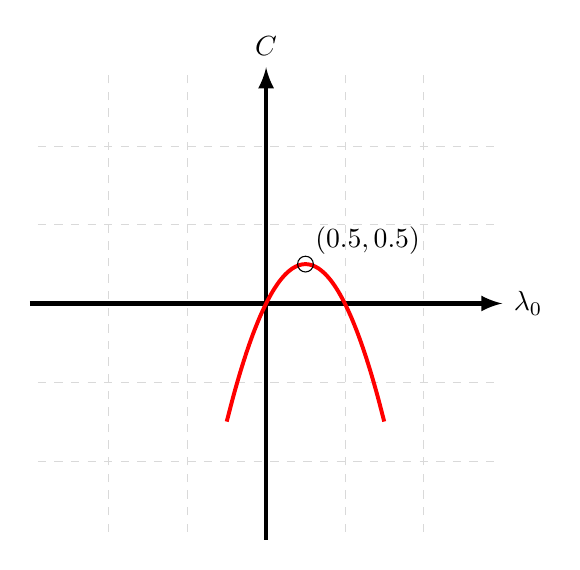
\begin{tikzpicture}
                    \draw[help lines, color=gray!30, dashed] (-2.9,-2.9) grid (2.9,2.9);
                    \draw[->,ultra thick] (-3,0)--(3,0) node[right]{$\lambda_0$};
                    \draw[->,ultra thick] (0,-3)--(0,3) node[above]{$C$};
                    \draw[red, line width = 0.50mm]   plot[smooth,domain=-0.5:1.5] (\x, {2*(\x-(\x)^2)});
                    \draw (0.5,0.5) circle (0.1)node[anchor=south west]{$(0.5, 0.5)$};
                    \end{tikzpicture}
                    }
                    \caption{Variation of concurrence $C$ of a quantum system with changing $\lambda_0$}
                    \label{fig:schmidtt-graph}
                \end{figure}

                % This yeilds the Schmidt Decomposition Theorem as
                % \begin{align*}
                %     \ket{\psi} &= \sum_{i,j=0}^1 x_{ij}\ket{i}\ket{j} \\
                %     x_{ij} &= \begin{bmatrix}\alpha & \beta \\ \gamma & \delta \end{bmatrix} \\
                %     \ket{\psi} &= (U_A \otimes U_B) (\lambda_0\ket{00} + \lambda_1\ket{11})
                % \end{align*}
                

        \subsection{Teleportation \& No Cloning Theorem}

        \subsection{Quantum Fourier Transform}
            \subsubsection{Binary Notation}
                First notice, one can represent a base 10 numbers in binary as follows:
            
                \begin{align*}
                    7_{10} &= 7 \ \text{base 10} \\
                    &= 0111_{2} \ \text{base 2}
                \end{align*}

                Therefore an $L$ qubit state can be represented as

                \begin{align*}
                L-\text{qubit state: } \ \ket{x} &= \ket{x_{L-1}} \otimes \ket{x_{L-2}} \otimes \cdots \otimes \ket{x_1}\otimes\ket{x_0}
                \end{align*}

                
            \subsubsection{Quantum Parallelism}
                Say one wants to evaluate function $f(x)$. In order for $f(x)$ to be a valid unitary it must be \textbf{bijective}. In order to evaluate a \textit{unitary}, you must use \textbf{two} registers.

                \begin{align*}
                \ket{x} \ (\text{L-qubits}) & \\
                \ket{y} \ (\text{M-qubits}) &: M\leq L \\
                &\longrightarrow U_f \ket{x}\ket{y} \\
                &= \ket{x}\ket{y\oplus f(x)}
                \end{align*}

                Note that this $\oplus$ is known as \textit{bit-wise addition modulo two} that is to say

                \begin{align*}
                0\oplus 0 &= 0\\
                1\oplus 0 &= 1\\
                0\oplus 1 &= 1\\
                1\oplus 1 &= 0\\
                1011 \oplus 0110 &= 10001 
                \end{align*}

                Therefore, one can evaluate a unitary $U_f$ as

                \begin{equation*}
                U_{f}\ket{y}\ket{x} = \ket{x}\ket{y\oplus f(x)\oplus f(x)} = \ket{x}\ket{y}
                \end{equation*}

                Since $f(x)$ alwasys evaluates to 0 or 1.

                Now to implement Quantum Parallelism one can do the following:

                \begin{align*}
                    H\ket{0}&=\frac{1}{\sqrt{2}}(\ket{0}+\ket{1}) \\
                    (H\otimes H)\ket{00} &= \frac{1}{2}(\ket{0}+\ket{1})(\cdots) \\
                    &= \frac{1}{2}(\ket{00}+\ket{01}+\ket{10}+\ket{11}) \\
                    \implies H^{\otimes L}\ket{0}_L &= \frac{1}{2^{\frac{L}{2}}} \sum_{x=0}^{2^L - 1}\ket{x} = \ket{a 11}_L
                \end{align*}


                Therefore, if we had the $H$ applied to all states in the argument register, we'd have

                \begin{align*}
                    (H^{\otimes L}\otimes I^{\otimes M})\ket{0}_L \otimes \ket{0}_M \ &\text{first ket is the arugment}\\
                    &= \ket{a11}_L\otimes\ket{0}_M \\
                    \implies U_f \ket{a11}_L\otimes \ket{0}_M &= \frac{1}{2^{\frac{L}{2}}}\sum_{x=0}^{2^L -1}\ket{x}\ket{f(x)}                  
                \end{align*}

            \subsubsection{Discrete Fourier Transform}
                First, note that \textit{any function that is periodic can be written as a sum of sines and cosines}. That is to say:
                \begin{align*}
                    f(t) &= \int_{-\infty}^{\infty} \tilde{f}(v)\exp(-2\pi i v t) \ dv \\
                    \tilde{f}(v) &= \int_{-\infty}^{\infty} f(t)\exp(2\pi i v t) \ dt
                \end{align*}

                Any statement that has a finite amount of energy can be written in such a manner. \textit{However,} when you do this on a computer, you cannot due infinitesimal calculations. So how is this done for a discrete case? Instead of functions, \textit{strings} are used, that is to say, \textit{sets of data} $\{f(t_0), f(t_1), f(t_2),\dots\}$. These will be a sample of the data points of the function at different points, $t_0, t_1, \dots$. This can be listed as follows:

                \begin{equation*}
                    \tilde{f}_{l} = \frac{1}{\sqrt{N}} \sum_{k=0}^{N-1}\exp(\frac{2\pi i k l}{N}f_k)
                \end{equation*}

                An example using the \texttt{DFT} is as follows. Say some function, $f_k$ as period $2$, and we evaluate $\tilde{f}_l$ using $N=7$ points, $\eta = \exp(2\pi i l / N)$.

                \begin{equation*}
                    \tilde{f_l} = \frac{1}{\sqrt{7}} (f_0 + f_1 \eta + f_2 \eta^2 + f_3 \eta^3 + f_4 \eta^4 + f_5 \eta^5 + f_6 \eta^6)
                \end{equation*}

                From this, we know that

                \begin{gather*}
                    f_6 = f_4  = f_2 = f_0 \\
                    f_5 = f_3 = f_1
                \end{gather*}

                Therefore, it follows that

                \begin{align*}
                \tilde{f_l} &= \frac{1}{\sqrt{7}} (f_0 + f_1 \eta + f_0 \eta^2 + f_1 \eta^3 + f_0 \eta^4 + f_1 \eta^5 + f_0 \eta^6) \\
                &= \frac{1}{\sqrt{7}}(f_0(1+\eta^2 + \eta^4) + f_1\eta(1+\eta^2 + \eta^4) + f_0\eta^6)\\
                &= \frac{1}{\sqrt{7}}(1+\eta^2 + \eta^4)(f_0 + f_1\eta) + \frac{f_0\eta^6}{\sqrt{7}}
                \end{align*}

                For arbitrary $N>7$, $\{f_0, f_1, \dots, f_{N-1}\}$. For some period $P$ we'd have
                \begin{gather*}
                    f_0 , f_1 , \dots , f_{P-1}, f_{P}, f_{P+1}, \\
                    \dots, f_{2P - 1}, f_{2P}, \dots, f_{3P-1}, f_{P+1}, \dots, f_{N} \\
                    \text{grouping these up} \\
                    (f_0 , f_1 , \dots , f_{P-1}), (f_{P}, f_{P+1}, \\
                    \dots, f_{2P - 1}), \\
                    (f_{2P}, \\\dots, f_{3P-1}), (f_{P+1}, \dots, f_{N})
                \end{gather*}
                Where each of these groupings represents one period of the target function. Writing this out in the DFT summation:
                \begin{equation} \label{eqn:DFT}
                \tilde{f}_l = \frac{1}{\sqrt{N}} \left(\sum_{k=0}^{P-1}f_k \eta^k\right)\left(\sum_{r=0}^{q-1}\eta^{Pr}\right) + \tilde{f_l}^{\text{end}} 
                \end{equation}
                Notice that the second summation is essentially a geometric progression with difference $r$. Therefore, this can be simplified to

                \begin{equation*}
                    \sum_{k=0}^{N-1} x^k = \frac{1-x^N}{1-x}
                \end{equation*}

                Since these need not be a \textbf{real} number, we can use this with our complex numbers in \eqref{eqn:DFT} to obtain:

                \begin{align*}
                \left(\sum_{r=0}^{q-1}\eta^{Pr}\right) &= \sum_{r=0}^{q-1}\exp(2\pi i (l/N)p)^r \\
                &= \frac{1-\exp(2 \pi i l p q / N)}{1 - \exp(2 \pi i l p / N)}
                \end{align*}

                Notice a problem, if $l,N\in \mathbb{Z}$ it implies that $\exp(2\pi i) = 1$. Therefore, if we substitute into the previous equation, we get a form $\frac{0}{0}$.

                \begin{mdframed}
                    \textit{This section is to be edited and corrected}
                \end{mdframed}

        \subsection{Algorithms}
            \subsubsection{Deutsch-Jozsa Algorithm}
                Consider a function $f(x)$ defined as:
                \begin{align*}
                    f(x) &= x \in\{0,1,\dots, 2^n - 1\} \ \texttt{n-bit arguement}\\
                    f(x) &= x \in\{0, 1\}
                \end{align*}

                The objective of the Deustch-Jozsa Algorithm \cite{deutsch_jozsa} is to determine whether $f(x)$ is either \textbf{constant} or \textbf{balanced}. That is to say, $f(x) = 0 \ \forall x$ **or** $f(x)=1 \ \forall x$ \textit{(constant function)} or $\texttt{equal number of 0 and 1}$ \textit{(balanced)}.

                Classically distinguishing between constant and balanced functions requires $2^{n-1}+1$ calls on the oracle.

                The algorithm can be represented using the circuit in figure \ref{fig:deustch-jozsa}

                \begin{figure}
                    \centering
                    \begin{quantikz}
                        \lstick{$\ket{0}$} & \qwbundle{n} \slice{$\ket{\psi_0}$} & \gate{H^{\otimes n}} \slice{$\ket{\psi_1}$} & \gate[2][2cm]{U_f}\gateinput{$x$}\gateoutput{$x$}\slice{$\ket{\psi_2}$}&\gate{H^{\otimes n}} \slice{$\ket{\psi_3}$} &\meter{} & \setwiretype{c}\\
                        \lstick{$\ket{1}$} && \gate{H} & \gateinput{$y$}\gateoutput{$y\oplus f(x)$} &&&
                    \end{quantikz}
                    \caption{Quantum Circuit diagram for representing the Deustch-Jozsa Algorithm for evaluating if a given binary function $f(x)$ is balanced}
                    \label{fig:deustch-jozsa}
                \end{figure}

                \begin{align*}
                    \ket{\psi_2} &= U_f \ket{\psi_1} \\
                    &= \sum_{x=0}^{2^n-1} \frac{\ket{x}}{\sqrt{2^n}}\left(\frac{\ket{f(x)}-\ket{\overline{f(x)}}}{\sqrt{2}}\right)\\
                    \implies U_f \ket{x}\ket{y} &= \ket{x}\ket{y\oplus f(x)} \\
                \end{align*}

                For a 1 qubit argument, $\ket{\psi_1}$ is easy to evaluate:

                \begin{align*}
                    H \ket{x} &= 
                        \begin{cases}
                            \frac{1}{\sqrt{2}} (\ket{0} + \ket{1})  &\text{if} \ x=0 \\
                            \frac{1}{\sqrt{2}} (\ket{0} - \ket{1}) &\text{if} \ x=1 
                        \end{cases} \\
                    &= \frac{(\ket{0}+ (-1)^x\ket{1})}{\sqrt{2}}
                \end{align*}

                Similarly, for a 2 qubit argument, on can evaluate $\ket{\psi_2}$. Notice that this is essentially multiplication modulo two.
                \begin{align*}
                (H\otimes H) \ket{x_1 x_0} &= \frac{(\ket{0}+ (-1)^{x_1}\ket{1})}{\sqrt{2}}\frac{(\ket{0}+ (-1)^{x_0}\ket{1})}{\sqrt{2}} \\
                &= \sum_{z=0}^3(-1)^{z_1 x_1 + z_0 x_0} \ket{z} \\
                \text{in general} &\implies H^{\otimes n}\ket{x} = \sum_{z=0}^{2^n-1}\frac{(-1)^{x\cdot z}\ket{z}}{\sqrt{2^n}} \\
                \implies x\cdot z &= (x_0z_0)\oplus (x_1 z_1)\oplus \cdots \oplus (x_{n-1}x_{n-1}) \\
                &= \bigoplus_{i=0}^{n-1}x_i z_i
                \end{align*}

                Finally one can extrapolate to the $n$-qubit case shown in figure \ref{fig:deustch-jozsa}. Say we have $\ket{\psi_3} = \left(H^{\otimes n}\otimes I\right)$ (note that $I$ is the unitary acting on the function register and $H$ is the unitary acting on the argument register). 

                \begin{align*}
                \ket{\psi_3} &= \left(H^{\otimes n}\otimes I\right) \\
                &= \left(\sum_{x,z=0}^{2^n -1}(-1)^{x\cdot z + f(x)}\ket{z}\right)\left\{\frac{\ket{0}-\ket{1}}{\sqrt{2}}\right\}\\
                &= \sum_{z=0}^{2^n-1}c_z\ket{z} \\
                \implies c_z &= \sum_{x=0}^{2^n - 1}\frac{(-1)^{z\cdot x + f(x)}}{2^n}
                \end{align*}

                As a test, Suppose that $f(x)$ is constant.

                \begin{align*}
                c_0 &\propto \left(\sum_{x=0}^{2^n - 1}\frac{1}{2^n}\right)(-1)^{f(0)} \\
                &\propto 1(-1)^{f(0)} \ \because \ \text{summation evaluates to} \ 1
                \end{align*}

                If all $n$ argument register quibts are in state $\ket{0}$ it implies that $f(x)$ is \textbf{constant}. If any qubit in the state $\ket{1}$ $f(x)$ must be \textbf{balanced}. This requires only 1 call on the oracle when classically it would require $2^n - 1$.

            \subsubsection{Bernstein-Vazariani Algorithm}

            \subsubsection{Grover's Algorithm}

            \subsubsection{Shor's Algorithm}

        \subsection{Quantum Error Correction}
            Let there by some arbitrary quantum state $\ket{\psi} = \alpha\ket{0} + \beta\ket{1}$. Inevitably the following will happen\footnote{Something like this bitflip error}:

        \begin{align*}
            \ket{\psi} = \alpha\ket{0} + \beta\ket{1} &\longrightarrow \ X\ket{\psi} = \beta\ket{0} + \alpha\ket{1}
        \end{align*}

        This ruins our algorithms, hence this begs the question, how cna you cope with an error like a bit flip in you $\Q$-Computer.

        \textit{Clue:}\textbf{ Classical Error Correction}, lets send 3 bits instead of one.
        \begin{align*}
            0 &\mapsto 000 \\
            1 &\mapsto 111
        \end{align*}

        Say there some bit flip error (could be one of the following)

        \begin{align*}
            000 &\longrightarrow 100, 010, 001 \\
            111 &\longrightarrow 011, 101, 110 
        \end{align*}

        Now here's a problem, what if two flip (screws everything up)? Well the has t do with the probability of an error occurring (square of error [dc with prof]).

        But now we have issues with error correction (in a quantum state), in order to do error correction you must measure a state thereby destroying it. Shor (and one other) showed this is not true and that \textbf{you can do error correction on a quantum state}.
            \subsection{Error Correcting Codes}
            \begin{figure}
                \centering
                \begin{quantikz}
                \lstick{$\ket{\varphi}$} & \qw & \ctrl{1} & \ctrl{2} &\gate{H}& \midstick[1]{Error} & \gate{H}& \\
                \lstick{$\ket{0}$} & \qw & \targ{1} & \qw & \gate{H} & \midstick[1]{Error} & \gate{H} &\\
                \lstick{$\ket{0}$} & \qw & \qw & \targ{1} & \gate{H} & \midstick[1]{Error} & \gate{H} &
                \end{quantikz}
                $\equiv$
                \begin{quantikz}
                \lstick{$\ket{\varphi}$} & \gate[3]{\chi} & \\
                \lstick{$\ket{0}$} & &\\
                \lstick{$\ket{0}$} & &
                \end{quantikz}
                \caption{Error Correction Circuit Intro}
                \label{fig:error-correction}
            \end{figure}

        Lets take the above with the state $\ket{\varphi} = \alpha\ket{000} + \beta\ket{111}$. The following are the possible errors.

        \begin{equation*}
            e(\ket{\varphi}) = \begin{cases}
                \alpha\ket{000} + \beta\ket{111} & \textit{Correct State} \\
                \alpha\ket{001} + \beta\ket{110} & \textit{Bitfip on} \ \Q_1 \\
                \alpha\ket{010} + \beta\ket{101} & \textit{Bitfip on} \ \Q_2\\
                \alpha\ket{100} + \beta\ket{011} & \textit{Bitfip on} \ \Q_3\\
            \end{cases}
        \end{equation*}

        Lets use a few auxiliary quits to correct.
        \begin{figure*}
            \centering
        \begin{quantikz}[column sep=1.3cm]
            \lstick{$\ket{\varphi}_5$} & \gate[3]{\chi}& \ctrl{5}\gategroup[6,steps=2,style={dashed,inner
sep=6pt}, label style={rotate=10, anchor=south, yshift=0.2cm}]{Flip anc. $\Q_0$ if $\Q_5\neq\Q_4$} &&\gategroup[6,steps=2,style={dashed,inner
sep=6pt}, label style={rotate=10, anchor=south, yshift=0.2cm}]{Flip anc. $\Q_2$ if $\Q_4\neq\Q_3$}&&\ctrl{4}\gategroup[6,steps=2,style={dashed,inner
sep=6pt}, label style={rotate=10, anchor=south, yshift=0.2cm}]{Flip anc. $\Q_1$ if $\Q_5\neq\Q_3$}&&  \\
            \lstick{$\ket{0}_4$} & && \ctrl{4} & \ctrl{2} &&&&\\
            \lstick{$\ket{0}_3$} & && &&\ctrl{1}&&\ctrl{2}&\\
            \lstick{$\ket{0}_2$} &&&&\targ{}&\targ{}&&&\rstick[3]{Ancillary $\Q$} \\
            \lstick{$\ket{0}_1$} &&&&&& \targ{} & \targ{} &\\
            \lstick{$\ket{0}_0$} && \targ{} & \targ{} &&&&&
        \end{quantikz}
        \caption{Full 3-bit error correction circuit using auxiliary qubit measurements to correct state. The \textbf{Ancillary $\Q$ (qubits) are the qubits used for error correction}. Qubit indices are explicitly denoted on the left of the diagram for clarity.}
            \label{fig:full-error}
        \end{figure*}

        %\gategroup[3,steps=8,label style={label position=below,anchor=north,yshift=-0.2cm}, background, style={fill=red!20}]{Ancillary (Error Correction) $\Q$s}&&& \targ{} & \targ{}

        %\gategroup[3,steps=3,style={inner sep=6pt}]{Ancillary (Error Correction) $\Q$s}

        Bit flip errors aren't actually all that common. Rather, time evolution is more of an issue. In fact this is a more likely scenario:

        \begin{align*}
            \ket{\phi} = \alpha\ket{0} + \beta\ket{0} &\rightarrow \alpha e^{i\epsilon}\ket{0} + \beta e^{-i\epsilon}\ket{1} \\
            &= \exp\{i\epsilon\hat{Z}\}\ket{\phi} \\
            &\approx \ket{\phi} + i\varepsilon \hat{Z}\ket{\psi}
        \end{align*}
            \subsection{Decoherence Free Spaces}

        \subsection{Quantum Key Distribution}

        \subsection{Device Physics}
            The device physics limits what you can implement experimentally. What do you actually need to make a quantum computer?
            \subsubsection{DiVincenzo's Requirements for a Physical Quantum Computer}
            \begin{enumerate}
                \item A lot of qubits
                \item must be able to initialize them (i.e. they have to be in the ground state $\ket{0}$, $\therefore$ they have to be very very cold)
                \item Must be reliable (you can have your probability amplitudes becoming \textit{decoherent}, i.e. $\alpha$ and $\beta$ become randomized). The time it takes for a state to experience \textit{decoherence} is \textbf{long}.
                \item Must be able to perform unitary operations/ quantum gates
                \item Must be able to measure them.
                
            \end{enumerate}

            \textit{This ``shopping list'' was made by David DiVincenzo in 2000}.

        \subsubsection{Methods of Physical Implementation}

            \begin{enumerate}
                \item Photons (1988)
                \item Ions (1994)
                \item Nuclear Spins (in molecules)
                \item Super conducting QuBits (currently lots of potential) \label{damn}
            \end{enumerate}

            From \ref{damn} we have a problem. We must engineer every single quantum system in a super conducting Qubit, it becomes a lot harder to fabricate. By definition every \texttt{Ca} atom is the same as every other \texttt{Ca} atom. 

            There is a \textit{bias} that more things should be solid state.

            Say we have a qubit in the following states

            \begin{gather*}
                \ket{\varphi} 
                \begin{cases}
                    \ket{0} & E_0 \\
                    \ket{1} & E_1
                \end{cases}
                \\
                E_1 - E_0 = \hbar\omega \\
                \ket{\phi} = A\ket{0} + B\ket{1}  \\
                \mathcal{H} = \begin{bmatrix} E_0 & 0 \\ 0 & E_1 \end{bmatrix} \\
                = I\left(\frac{E_0+E_1}{2}\right) + \frac{\hbar\omega}{2}Z
            \end{gather*}

        \subsubsection{Temperature Bound}
            Notice the Maxwell-Boltzman Distribution 
            \begin{align*}
                p_n \propto \exp{-E_n / k_B\theta_T}
            \end{align*}

            Therefore it follows that the probability of being in a state $p_1/p_0$ is 
            \begin{align*}
                p_1 / p_0 &= \exp{-(E_1-E_0)/k_B\theta_T} \\
                &= \exp{-\hbar\omega/k_B\theta_T} \\
                &\ll 1 \implies \frac{\hbar\omega}{k_B\theta_T} \gg 1 \\
                &\therefore \theta_T \ll  \frac{\hbar\omega}{k_B}
            \end{align*}

        \subsubsection{Time Evolution}
            Notice the Schr{\"o}dinger equation
            \begin{equation}
                i\hbar\pdv{}{t}\ket{\phi} = \mathcal{H}\ket{\phi}
            \end{equation}

            Therefore it follows that 
            \begin{align*}
                i\hbar\pdv{}{t} A &= E_0 A \\
                \implies A(t) &= A(0)\exp{-iE_0 t / \hbar} \\
                i\hbar\pdv{}{t} B &= E_1 B \\
                \implies B(t) &= B(0)\exp{-iE_1 t / \hbar}
            \end{align*}

            We see then that our coefficients $A$ and $B$ will be \textbf{constantly changing in time} as follows

            \begin{align*}
                \ket{\phi(t)} &= A(0)e^{\frac{-i E_0 t}{\hbar}}\ket{0} + B(0)e^{\frac{-i E_1 t}{\hbar}}\ket{1} \\
                &= \exp\left(-i\frac{(E_0 + E_1)t}{\hbar}\right)\left\{A(0)e^{\frac{i \omega t}{\hbar}}\ket{0} + B(0)e^{\frac{-i\omega t}{\hbar}}\ket{1}\right\} \tag{$\star$}\label{eqn:bingpot}
            \end{align*}

            The first term is the \textit{global phase} and can be ignored for our purposes.

            \eqref{eqn:bingpot} can be rewritten using Euler's formula

            \begin{equation*}
                A(0)\{\cos(\omega t/2) + i\sin(\omega t/2)\}\ket{0} + B(0)\{\cos(\omega t/2) - i\sin(\omega t/2)\}\ket{1}
            \end{equation*}

            It then follows as a unitary

            \begin{align*}
                U_0(t) &= \cos(\omega t/2)I + i\sin(\omega t / 2) Z \\
                \implies \ket{\phi(t)} = U_0 (t)\ket{\phi(0)}
            \end{align*}

            \textbf{That means the operators must also change in time as well!!!}

            Therefore it follows that 

            \begin{align*}
                \bra{\zeta}X\ket{\varphi} = (\bra{\zeta}U_0^\dagger)U_0 X U_0^\dagger (U_0\ket{\varphi})
            \end{align*}

            \begin{enumerate}
                \item Energy gap between $\ket{0}$ and $\ket{1}$ ($E_0$ and $E_1$, $\hbar\omega=E_1-E_0$).
                \begin{enumerate}
                    \item Temperature must be $T\ll \frac{\hbar\omega}{k_B}$
                    \item Driver Synchronization $\omega_d = \omega$
                \end{enumerate}
                \item Single Qubit Gates can be implemented using a \textit{time-harmonic force} $\vec{f}(t)=\vec{f_0}\cos(\omega t + \phi)$.
                \begin{equation*}
                    \hat{U}(t) = \cos\left(\frac{\Omega t}{2}\right)\hat{I} - i\sin\left(\frac{\Omega t}{2}\right)\{\cos\phi\hat{X} + \sin\phi\hat{Y}\}
                \end{equation*}
                \begin{enumerate}
                    \item Rabi Oscillations $\Omega \propto f_0$
                    \item $\Omega t = \pi$ ``pi-pulse'' which means (substitute into equation)
                    \begin{equation*}
                        \hat{U}\left(\frac{\pi}{\Omega}\right) = -i\{\cos\phi\hat{X} + \sin\phi\hat{Y}\}
                    \end{equation*}
                    \item $\therefore \ \text{Pauli Gates} \ \implies \pi-\text{pulse}$
                    \item $\Omega t = \pi/2, \phi = \frac{3\pi}{2}$ ``pi-upon-two-pulse'' which means (substitute into equation)
                    \begin{equation*}
                        \hat{U} = \frac{1}{\sqrt{2}}(\hat{I} + i\hat{Y}) = i\hat{H}
                    \end{equation*}
                    \item $\Omega t = 2\pi$ Allows you to make $\hat{U} = -\hat{I}$
                \end{enumerate}
                \item Two qubit gates (two methods)
                \begin{enumerate}
                    \item Method (1)
                    \begin{enumerate}
                        \item Remember they are two physical entities
                        \begin{figure}
                        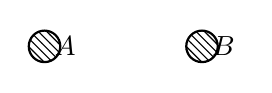
\begin{tikzpicture}
                            \draw[thick, pattern=north west lines] (-1,0)node[anchor=west]{$A$} circle (0.2);
                            \draw[thick, pattern=north west lines] (1,0)node[anchor=west]{$B$} circle (0.2);
                        \end{tikzpicture}
                        \end{figure}
                        Therefore it follows that they \textit{will} interact as defined in the Schr{\"o}dinger equation.
                        \begin{equation*}
                            i\hbar\pdv{}{t}\ket{\Phi_{AB}} = \{\}
                        \end{equation*}
                    \end{enumerate}
                \end{enumerate}
            \end{enumerate}
            % \subsubsection{Single Qubit Control}
            
            % \subsubsection{Short Range Qubit-Qubit Control}
            
            % \subsubsection{Long Range Qubit-Qubit Control}
            

    \section{Problem Set Questions}
        \subsection{Problem Set One}
            \subsubsection{Question One: Eigenvalues and Properties of Pauli Matrices}
                \paragraph{Question:}
                
                The three \textit{Pauli matrices} are given by:
                \begin{equation*}
                    \hat{X} = \begin{bmatrix}0 & 1 \\1 & 0\end{bmatrix}, \
                    \hat{Y} = \begin{bmatrix}0 & -i \\i & 0\end{bmatrix}, \
                    \hat{Z} = \begin{bmatrix}1 & 0 \\0 & -1\end{bmatrix}
                \end{equation*}

                Find the eigenvectors, eigenvalues, and diagonal representations of $\hat{X}$, $\hat{Y}$, and $\hat{Z}$.

                \begin{mdframed}
                    \paragraph{Answer:}

                    
                \end{mdframed}
                
            \subsubsection{Question Two: Playing with Pauli Matrices}
                \paragraph{Question:}
                
                Show that:
                \begin{equation*}
                    \hat{X}\hat{Y} = i\hat{Z}, \ \hat{Y}\hat{Z} = i\hat{X}, \ \hat{Z}\hat{X} = i\hat{Y}
                \end{equation*}

                And hence $\hat{X}\hat{Z}\hat{X} = -\hat{Z}$

                \begin{mdframed}
                    \paragraph{Answer:}

                    
                \end{mdframed}

            \subsubsection{Question Three: Verifying a Matrix is Unitary}
                \paragraph{Question:}
                
                A \textit{unitary matrix} is a matrix whose inverse is equal to its Hermitian adjoint (i.e take the transpose and the complex-conjugate). Show that 
                \begin{equation*}
                    \hat{U} = \begin{bmatrix}a & b \\ -b^* & a^*\end{bmatrix}
                \end{equation*}

                (where $|a|^2 + |b|^2 = 1$) is unitary.

                \begin{mdframed}
                    \paragraph{Answer:}

                    
                \end{mdframed}


        \subsection{Problem Set 2}
            \subsubsection{Question One: Looking at the Bloch Sphere}
                \paragraph{Question:}
                
                The \textit{Bloch vector} is alternative way to represent the state of a qubit in a real three-dimensional space $\mathbb{R}^3$ (rather than a complex two-dimensional space $\mathbb{C}^2$). It is defined by 
                \begin{equation*}
                    S_i = \bra{\varphi}\hat{\sigma_i}\ket{\varphi}
                \end{equation*}

                where $\hat{\sigma_i}$ ($i=1,2,3$) are the Pauli matrices.
                
                \begin{itemize}
                    \item[(a)] Show that for states given by a properly normalized vector in $\mathbb{C}^2$, the Bloch vector is a real unit vector (i.e. $\sum\limits_{i=1}^{3}S_i^2 = 1$)
                    \item[(b)] Work out the components of the Bloch vector for the following states 
                        \begin{enumerate}
                            \item[(i)] $\ket{0}$
                            \item[(ii)] $\ket{1}$
                            \item[(iii)] $\frac{1}{\sqrt{2}}(\ket{0}+\ket{1})$
                            \item[(iv)] $\frac{1}{\sqrt{2}}(\ket{0}+i\ket{1})$
                        \end{enumerate}
                    \item[(c)] The \textit{Kronecker Product} (also called the \textit{outer product}) of two vectors $\ket{\psi} = a\ket{0} + b\ket{1}$ and $\ket{\phi} = c\ket{0} + d\ket{1}$ in a two-dimensional Hilbert space is a 2x2 matrix defined by 
                        \begin{equation*}
                            \ket{\psi}\bra{\phi} = \begin{bmatrix}a \\ b\end{bmatrix} \begin{bmatrix}c^* & d^*\end{bmatrix} = \begin{bmatrix}ac^* & ad^* \\ bc^* & bd^*\end{bmatrix}
                        \end{equation*}
                        \begin{itemize}
                            \item[(i)] Find the eigenvalues of $\ket{\psi}\bra{\psi}$
                            \item[(ii)] Show that $\ket{\psi}\bra{\psi} = \frac{1}{2}(\hat{I}+\mathbf{S}\cdot\mathbf{\hat{\sigma}})$ (where $\mathbf{S}\cdot\mathbf{\hat{\sigma}} = \sum\limits_{i=1}^3 S_i\hat{\sigma}_i$)
                        \end{itemize}
                \end{itemize}

                \begin{mdframed}
                    \paragraph{Answer:}

                    
                \end{mdframed}
                
            \subsubsection{Question Two: Unitary Operations on the Bloch Sphere}
                \paragraph{Question:}
                
                Now let's consider the effect of unitary operations on the Bloch vector. 
                \begin{itemize}
                    \item[(a)] Show that the operator given by the following expression is unitary
                    \begin{equation*}
                        \hat{U} = \cos{\frac{\theta}{2}}\hat{I} + i\sin{\frac{\theta}{2}}\mathbf{n}\cdot\mathbf{\hat{\sigma}}
                    \end{equation*}
                    where $\mathbf{n}$ is a real unit vector.
                    \item[(b)] If $\ket{\varphi'} = \hat{U}\ket{\varphi}$, show that the transformed Bloch vector $\mathbf{S}' = \bra{\varphi'}\mathbf{\hat{\sigma}}\ket{\varphi'}$ is the original Bloch vector rotated by an angle $\theta$ about an axis along the unit vector $\mathbf{n}$, i.e.:
                    \begin{equation*}
                        \mathbf{S}' = \cos\theta\mathbf{S} + (1-\cos\theta)(\mathbf{n}\cdot\mathbf{S})\mathbf{n}-\sin\theta(\mathbf{n}\times\mathbf{S})
                    \end{equation*}
                \end{itemize}

                \begin{mdframed}
                    \paragraph{Answer:}

                    
                \end{mdframed}

        \subsection{Problem Set 3}
            \subsubsection{Question One: Evaluating Concurrence}
                \paragraph{Question:}
                    Consider the following 2-qubit state
                    \begin{equation*}
                        \ket{\phi} = \frac{1}{10}\{i\sqrt{27}\ket{00} + 3\ket{01} - 4\ket{10}-i\sqrt{48}\ket{11}\}
                    \end{equation*}

                    \begin{itemize}
                        \item[(a)] Is the state entangled? If so, calculate its concurrence.
                        \item[(b)] Calculate the Schmidt numbers of the state
                    \end{itemize}

                    \begin{mdframed}
                    \paragraph{Answer:}

                    \subparagraph{Part (a)}
                        Using \eqref{eqn:concurence}, 
                        \begin{align*}
                            C &= 2|\alpha\delta - \beta\gamma| \\
                            &= 2\left| \frac{(i\sqrt{27})\cdot (-i\sqrt{48}) - (3)\cdot(-4)}{100}\right| \\
                            &= \frac{1}{50}\left|3\sqrt{3}\cdot4\sqrt{3} +12 \right| \\
                            &= \frac{48}{50} \\
                            &= 0.96
                        \end{align*}

                        Therefore the state \textbf{is entangled with a concurrence of $C=96\%$}

                    \subparagraph{Part (b)}
                        From Theorem \ref{thm:schmidt} we have \eqref{eqn:schmidtt-2}

                        \begin{align*}
                            \lambda^2 &= \frac{1\pm\sqrt{1-C^2}}{2} \\
                            &= \frac{1\pm 0.28}{2} \\
                            \implies \lambda_0 = \sqrt{0.64}=0.8;& \ \lambda_1  = \sqrt{0.36}=0.6
                        \end{align*}
                    
                    \end{mdframed}
            \subsubsection{Question Two: The \texttt{SWAP} gate}
                \paragraph{Question:}
                    The \texttt{SWAP} gate swaps the states of the two qubits, so that:
                    \begin{equation*}
                        \texttt{SWAP}(\alpha\ket{00}+\beta\ket{01}+\gamma\ket{10}+\delta\ket{11}) = \alpha\ket{00}+\gamma\ket{01}+\beta\ket{10}+\delta\ket{11}
                    \end{equation*}

                    \begin{itemize}
                        \item[(a)] Write down the 4x4 matrix for \texttt{SWAP}
                        \item[(b)] Can you write the \texttt{SWAP} gate as local operations on the two qubits? \textit{Hint: try writing out the block-matrix for $\hat{U}_1\otimes\hat{U}_2$ and comparing it to the matrix form for \texttt{SWAP}}
                        \item[(c)] Can \texttt{SWAP} be used to create entanglement? If so, write out the quantum circuit.
                        \item[(d)] Derive an expression $\sqrt{\texttt{SWAP}}$, defined by $\sqrt{\texttt{SWAP}}\sqrt{\texttt{SWAP}} = \texttt{SWAP}$
                        \item[(e)] Can $\sqrt{\texttt{SWAP}}$ be used to create entanglement? Find a separable state that will become maximally entangled when $\sqrt{\texttt{SWAP}}$ is applied to it.
                    \end{itemize}

                \begin{mdframed}
                    \paragraph{Answer:}

                    
                \end{mdframed}

        \subsection{Problem Set 4}
            \subsubsection{Question One: Proving Circuit Identities}
                \paragraph{Question:}
                Prove the following quantum circuit identities
                \begin{itemize}
                    \item[(a)]
                        \begin{quantikz}
                            & \gate{X} & \ctrl{1} & \\
                            & & \targ{1} & 
                        \end{quantikz}
                        $=$
                        \begin{quantikz}
                            & \ctrl{1} & \gate{X} &\\
                            & \targ{1} & \gate{X} &
                        \end{quantikz}
                    \item[(b)]
                        \begin{quantikz}
                            & \ctrl{1} & \gate{X} & \ctrl{1} & \\
                            & \targ{1} & & \targ{1} 
                        \end{quantikz}
                        $=$
                        \begin{quantikz}
                            & \gate{X} &\\
                            & \gate{X} &
                        \end{quantikz}

                    \item[(b)]
                        \begin{quantikz}
                            & \ctrl{1} & & \ctrl{1} & \\
                            & \targ{1} & \gate{X} & \targ{1} 
                        \end{quantikz}
                        $=$
                        \begin{quantikz}
                            & &\\
                            & \gate{X} &
                        \end{quantikz}
                \end{itemize}
            
                \begin{mdframed}
                \paragraph{Answer:}
                \end{mdframed}

            \subsubsection{Question Two: The Griffiths-Niu Theorem}
                \paragraph{Question:} \textbf{Griffiths-Niu Theorem} Given two qubits $A$ and $B$, show that, if a measurement is performed on $A$ followed by a conditional application of a unitary, $\hat{U}$, on $B$ then the resultant state is equivalent to a controlled-$\hat{U}$ gate on $B$ followed by a measurement on $A$ (see figure).
                \begin{center}
                    \begin{quantikz}
                        & \meter{} & \ctrl[vertical wire=c]{1}\setwiretype{c} \\
                        & &\gate{U}\wire[u][1]{c}
                    \end{quantikz}
                    $\equiv$
                     \begin{quantikz}
                        & \ctrl{1} & \meter{} & \setwiretype{c} \\
                        & \gate{U} & &
                    \end{quantikz}
                \end{center}
                \begin{mdframed}
                \paragraph{Answer:}

                
                \end{mdframed}
            \subsubsection{Question Three: Simplifying The Quantum Teleportation Circuit}
                \paragraph{Question:} \textbf{Circuit-Based Proof for Teleportation} Here is the full teleportation circuit discussed in class:
                \begin{center}
                \begin{quantikz}
                \lstick{$\ket{\varphi}$} \slice{$\ket{\psi_{0}}$} & &\slice{$\ket{\psi_{1}}$} & \ctrl{1} & \gate{H}\slice{$\ket{\psi_{2}}$} & \meter{} & \setwiretype{c} & \ctrl[vertical wire=c]{0} \\
                \lstick{$\ket{0}$} & \gate{H} & \ctrl{1} & \targ{1} & & \meter{}&\ctrl{0} \setwiretype{c}  \\
                \lstick{$\ket{0}$} & & \targ{1} & & & &\gate{X}\wire[u][1]{c} &\gate{Z}\wire[u][2]{c} & 
                \end{quantikz}
                \end{center}
                \begin{itemize}
                    \item[(a)] Use the Griffiths-Niu Theorem to show that the teleportation circuit has the same effect as the circuit below.
                    \begin{center}
                        \begin{quantikz}
                        \lstick{$\ket{\varphi}$} \slice{$\ket{\psi_{0}}$} & &\slice{$\ket{\psi_{1}}$} & \ctrl{1} & \gate{H}\slice{$\ket{\psi_{2}}$} &&\ctrl{2} \slice{$\ket{\psi_{3}}$}& \meter{} & \setwiretype{c}  \\
                        \lstick{$\ket{0}$} & \gate{H} & \ctrl{1} & \targ{1} & & \ctrl{1}&&\meter{} &\setwiretype{c} \\
                        \lstick{$\ket{0}$} & & \targ{1} & & & \targ{1} & \gate{Z}\wire[u]{1}{c} & &
                        \end{quantikz}
                    \end{center}
                    \item[(b)] Use the identity $\hat{H}\hat{X}\hat{H}=\hat{Z}$ to rewrite the appropriate part of the circuit
                    \begin{center}
                        \begin{quantikz}
                            & \ctrl{2} & \\
                            & & \\
                            & \gate{Z}\wire[u]{2}{c} &
                        \end{quantikz}
                        $=$
                        \begin{quantikz}
                            & \gate{Z}\wire[u]{2}{c} & \\
                            & & \\
                            & \ctrl{-2} &
                        \end{quantikz}
                        $=$
                        \begin{quantikz}
                            & \gate{H} & \targ{} & \gate{H} & \\
                            &&&& \\
                            &&\ctrl{-2}&&
                        \end{quantikz}
                    \end{center}
                    \item[(c)] Use $\hat{H}\hat{H} = \hat{I}$ and the fact that $\hat{H}\ket{0}$ is an eigenstate of $\hat{X}$ to add another \texttt{CNOT} (whose significance will soon be apparent).
                    \item[(d)] Work out what appropriate single \texttt{CNOT} gate replaces the \texttt{CNOT} gate combination below:
                    \begin{center}
                        \begin{quantikz}
                            & \ctrl{1} && \ctrl{1} && \\
                            & \targ{} & \ctrl{1} & \targ{} & \ctrl{1} & \\
                            && \targ{} && \targ{} &
                        \end{quantikz}
                    \end{center}
                    \item[(e)] Apply what you found in (d) on the teleportation ciruit to simplify it furter; this is what it should be looking like by now:
                    \begin{center}
                        \begin{quantikz}
                        \lstick{$\ket{\varphi}$} && \ctrl{2}&\targ{}&\gate{H} &\meter{} & \setwiretype{c}  \\
                        \lstick{$\ket{0}$} & \gate{H} &&& &\meter{} &\setwiretype{c} \\
                        \lstick{$\ket{0}$} &&\targ{}&\ctrl{-2}&&&
                        \end{quantikz}
                    \end{center}
                    \item[(f)] You fill find that qubit \#2 will no longer by involved in any multi-qubit gates. In other words, it has become a \textit{spectator} qubit. Move the Hadamard gate acting on this qubit all the way to the right just before measurement.
                    \item[(g)] Make a \texttt{SWAP} gate by creating a combination of \texttt{CNOT} gate (remember question 2 of hte Term Test), acting on qubits \#3 and \#1, by inserting a \texttt{CNOT} gate with qubit \#1 being the control qubit. Since qubit C is in a state $\ket{0}$, that will have no effect. You should end up with the circuit shown below:
                    \begin{center}
                        \begin{quantikz}
                        \lstick{$\ket{\varphi}$} & \swap{2} & \gate{H} & \meter{} & \setwiretype{c} \\
                        \lstick{$\ket{0}$} & & \gate{H} & \meter{} & \setwiretype{c}\\
                        \lstick{$\ket{0}$} & \targX{} &&& \rstick{$\ket{\varphi}$}
                        \end{quantikz}
                    \end{center}
                \end{itemize}

                \begin{mdframed}
                \paragraph{Answer:}

                
                \end{mdframed}

        \subsection{Problem Set 5}
            \subsubsection{Question One: Introduction to Oracles}
                \paragraph{Question:}
                The \textit{bit-by-bit modulo-2 product} of two L-bit integers $a$ and $b$ is defined as 
                \begin{equation*}
                    a\cdot b = (a_{L-1}b_{L-1})\oplus (a_{L-2}b_{L-2})\oplus\dots\oplus(a_1b_1)\oplus(a_0b_0)
                \end{equation*}

                where $a_k$ is the value of hte $k$-th binary digit when $a$ is written in base 2 (and likewise for $b$); $\oplus$ is addition modulo 2 (i.e. add the two numbers, then calculate the remainder when dviding by 2).

                \begin{itemize}
                    \item[(a)] If $a=5$ and $b=6$ (both in base 10), find $a\cdot b$
                    \item[(b)] Prove that, in general, $a\cdot b\neq ab \mod 2$
                    \item[(c)] Prove that, for two qubits, $\texttt{CNOT}\ket{x,y}=\ket{x, y\oplus x}$ (where the first qubit is the control and the second the target of the \texttt{CNOT}, and $x$ and $y$ can both take the values of 0 or 1).
                    \item[(d)] Let $f(x) = a\cdot x$, where $a$ is some unknown constant. Defining the oracle operator in the usual way (i.e. $\hat{U}_f\ket{x}\ket{y} = \ket{x}\ket{y\oplus f(x)}$), show that the output of the following quantum circuit yields the value of $a$.
                    \begin{center}
                        \begin{quantikz}
                            \lstick{$\ket{0}^{\otimes L}$} & \qwbundle{L} & \gate{H^{\otimes L}} & \gate[2]{U_f} & \gate{H^{\otimes L}} & \meter{} &\setwiretype{c}\\
                            \lstick{$\ket{0}$} & \gate{X} & \gate{H} &&&&
                        \end{quantikz}
                    \end{center}
                    \textit{Hint: you may use the identity $H^{\otimes L}\ket{y}=\frac{1}{\sqrt{2^L}}\sum\limits_{n=0}^{2^L-1}(-1)^{x\cdot y}\ket{y}$ without proof.}
                \end{itemize}

                \begin{mdframed}
                \paragraph{Answer:}

                
                \end{mdframed}

            \subsubsection{Question Two: Using Qubit to Store Binary}
                \paragraph{Question:} \textbf{Qubit registers as classical data storage devices} Let $x$ be a 3-bit number with binary digits $\{x_0,x_1,x_2\}$, i.e. $x=\sum\limits_{n=0}^{2}x_n2^n$. This number can be represented as a quantum state of two qubits as follows:
                \begin{equation*}
                    \ket{\psi(x)} = \frac{1}{2}(\ket{11}+\zeta_2\ket{10} + \zeta_1\ket{01}+\zeta_0\ket{00})
                \end{equation*}

                where $\zeta_n = 2x_n - 1$ (i.e. the bits of $x$ stored in the phases of the probability amplitudes of the computational basis states, with phase $\phi_n=0$ corresponding to $x_n=1$ and $\phi_n=\pi$ corresponding to $x_n=0$)
                \begin{itemize}
                    \item[(a)] Why cannot we use the probability amplitude of the state $\ket{11}$ to store a forth bit?
                    \item[(b)] Devise simple quantum circuits to store the following numbers:
                        \begin{itemize}
                            \item[(i)] $x = 7$
                            \item[(ii)] $x = 3$
                            \item[(iii)] $x = 4$
                        \end{itemize}
                    \item[(c)] It has been estimated that all the information stored in all of the electronic data storage technology world-wide amounts to about $1.4 \cdot 1024$ bits. If we decided to encode this information in a multi-qubit state, now many qubits would be needed?
                    \item[(d)] {\`A} propos the previous question, why would such an approach to data storage be of dubious utility?
                \end{itemize}

                \begin{mdframed}
                \paragraph{Answer:}

                
                \end{mdframed}

        \subsection{Problem Set 6}
            \subsubsection{Question One: Using the Discrete Fourier Transform}
                \paragraph{Question:} Find, simplify and plot the \textit{Discrete Fourier Transform} of the following sequences analytically:
                \begin{itemize}
                    \item[(a)] $\{0,1,0,1\}$
                    \item[(b)] $\{0,1,2,0,1,2,0,1,2\}$
                    \item[(c)] $\{0,4,2,0,4,2,0,4\}$
                \end{itemize}

                \begin{mdframed}
                \paragraph{Answer:}

                
                \end{mdframed}

            \subsubsection{Question Two: Finding and Plotting Frequencies using the Discrete Fourier Transform}
                \paragraph{Question:}
                \begin{itemize}
                    \item[(a)] Consider the array of $N = 12$ values of a function of period $p = 4$:
                    \begin{equation*}
                        f_k = \{-3, 1, -1, 3, -3, 1, -1, 3, -3, 1, -1, 3\}
                    \end{equation*}
                    Numerically calculate the Discrete Fourier Transform and plot $|\tilde{f_l}|$ for $l= 0, 1,\dots 11$.
                    \item[(b)] Now consider the array of $N = 14$ values of the same function
                    \begin{equation*}
                        f_k = \{-3, 1, -1, 3, -3, 1, -1, 3, -3, 1, -1, 3, -3, 1\}
                    \end{equation*}
                    Numerically calculate the Discrete Fourier Transform and plot $|\tilde{f_l}|$ for $l= 0, 1,\dots 13$.
                \end{itemize}

                \begin{mdframed}
                \paragraph{Answer:}

                
                \end{mdframed}

            \subsubsection{Question Three: The Quantum Fourier Transform}
                \paragraph{Question:} 
                The Quantum Fourier Transform on $n$ qubits is defined by
                \begin{equation*}
                    \hat{U}_{QFT}\ket{l} = \frac{1}{\sqrt{2^n}}\sum\limits_{k=0}^{2^n-1}\exp{2\pi i\frac{kl}{2^n}}\ket{k}
                \end{equation*}
                Prove $\hat{U}_{QFT}$ is unitary.

                \begin{mdframed}
                \paragraph{Answer:}

                
                \end{mdframed}

        \subsection{Problem Set 7}
             \subsubsection{Question One: Generalizing Controlled Unitaries}
                \paragraph{Question:} 
                Prove the following quantum circuit identity:
                \begin{center}
                    \begin{quantikz}
                        & & \ctrl{1} &&& \ctrl{1} & & \\
                        &\gate{U} & \targ{} & \gate{U^\dagger} & \gate{V} & \targ{} & \gate{V^\dagger}
                    \end{quantikz}
                    $=$
                    \begin{quantikz}
                        & \ctrl{1} & \\
                        & \gate{V^\dagger X V U^\dagger X U} &
                    \end{quantikz}
                \end{center}
                where $U$ and $V$ are unitary operators.  Prove that any unitary operator can be expressed in the form $V^\dagger X V U^\dagger X U$  (thus this circuit allows \textit{any} controlled unitary to be performed using local unitaries and \texttt{CNOT}s.
            \subsubsection{Question Two: Generalizing Unitaries Analytically}
                \paragraph{Question:} 
                Let $\hat{U}(\theta) = \cos{\frac{\theta}{2}}\hat{I} + i\sin{\frac{\theta}{2}}\hat{Z}_0$, where $\hat{I}$ and $\hat{Z}_0$ is the standard ($\theta$-independent) Pauli operator (similarly for $\hat{X}_0$ and $\hat{Y}_0$ below). Find:
                \begin{itemize}
                    \item[(a)] $\hat{X}(\theta) = \hat{U}(\theta) \hat{X}_0\hat{U}^\dagger(\theta)$ \textit{Hint: slogging through the matrix multiplication will get you there, but it might be quicker to use $\hat{Z}_0\hat{X}_0 = -\hat{X}_0\hat{Z}_0$, (which implies $\hat{Z}_0\hat{X}_0\hat{Z}_0 = -\hat{X}_0$), and $[\hat{Z}_0, \hat{X}_0]=i2\hat{Y}_0$
                    \item[(b)] $\hat{Y}(\theta) = \hat{U}(\theta) \hat{Y}_0\hat{U}^\dagger(\theta)$
                    \item[(c)] $\hat{Z}(\theta) = \hat{U}(\theta) \hat{Z}_0\hat{U}^\dagger(\theta)$}
                    \item[(d)] Suppose one could implement $\hat{X}(\theta)$ for an arbitrary value of $\theta$. How would use use it to implement the following (If you can't find a solution, try proving it's impossible instead):
                    \begin{itemize}
                        \item[(i)] $\hat{Y}_0$
                        \item[(ii)] $\hat{Z}_0$
                        \item[(iii)] The Hadamard gate $\hat{H}$
                    \end{itemize}
                \end{itemize}

                \begin{mdframed}
                \paragraph{Answer:}

                
                \end{mdframed}
                
        \subsection{Problem Set 8}
            \subsubsection{Question One: Time Dependence in Quantum Information}
                We saw in class that realistic physical qubits are continuously evolving in time, so that the state of a single qubit is $\ket{\phi(t)} = A(t)\ket{0} + B(t)\ket{1}$. Here we are going to consider the case of single qubit operations in which the drive frequency is slightly detuned from the qubit resonance frequency. Let $\omega = \frac{E_1 - E_0}{\hbar}$ be the natural frequency of the qubit; when an external force, oscillating at frequency $\omega_d$, is applied, the amplitudes $A(t)$ and $B(t)$ obey the following differential equations:
                    \begin{align*}
                        i\dot{A} &= -\frac{\omega}{2} A - \Omega_0 \cos(\omega_d t) B \\
                        i\dot{B} &= -\frac{\omega}{2} B - \Omega_0 \cos(\omega_d t) A
                    \end{align*}
                where $\dot{A}$ is the time derivative of $A(t)$, and $\Omega_0$ is a constant with units of frequency, and proportional to the strength of the applied force.

                \begin{itemize}
                    \item[(a)] Introducing the new variables $\alpha(t) =\exp(-i\omega_dt/2)A(t)$  and$\beta(t) = \exp(i\omega_dt/2)B(t)$, and using the rotating wave approximation, show that $\alpha(t)$ and $\beta(t)$ obey the following time-independent equations:
                        \begin{align*}
                            i\dot{\alpha} &= \frac{\Delta \alpha + \Omega_0 \beta}{2} \tag{A}\label{eqn:ps8q1-a}\\
                            i\dot{\beta} &= \frac{-\Delta \beta + \Omega_0 \alpha}{2} \tag{B}\label{eqn:ps8q1-b}
                        \end{align*}
                    where $\Delta = \omega_d - \omega$
                    \item[(b)] By differentiating \eqref{eqn:ps8q1-a} and substituting from \eqref{eqn:ps8q1-a} and \eqref{eqn:ps8q1-b}, one can obtain a simple second-order ordinary differential equation for $\alpha$. By solving this equation (and the similar equation for $\beta$), show that
                        \begin{equation*}
                            \begin{bmatrix} \alpha(t)\\\beta(t)\end{bmatrix} = \hat{U}(t)\begin{bmatrix}\alpha(0)\\ \beta(0)\end{bmatrix}
                        \end{equation*}
                    where $\hat{U}(t) = \cos(\omega t/2)\hat{I} - i\sin(\Omega t/2)\{\Delta\hat{Z} - \Omega_0\hat{X}\}/\Omega, and \Omega = \sqrt{\Omega_0^2+\Delta^2}$
                \end{itemize}

                \begin{mdframed}
                \paragraph{Answer:}

                
                \end{mdframed}

            \subsubsection{Question Two: Solving the Equations of Motion for Quantum States}
                \paragraph{Question:} The evolution of the state $\ket{\varphi_{AB}(t)} = \alpha(t)\ket{00} + \beta(t)\ket{01} + \gamma(t)\ket{10} + \delta(t)\ket{11}$ of two interacting qubits has the following form:
                \begin{equation*}
                    i\hbar\pdv{}{t}
                    \begin{bmatrix}
                    \alpha\\\beta\\\gamma\\\delta
                    \end{bmatrix} 
                    = \hbar\Omega_0
                    \begin{bmatrix}
                        1 & 0 & 0 & 0 \\
                        0 & -1 & w & 0 \\
                        0 & w & -1 & 0 \\
                        0 & 0 & 0 & 1
                    \end{bmatrix}
                    \begin{bmatrix}
                        \alpha \\ \beta \\ \gamma \\ \delta 
                    \end{bmatrix}
                \end{equation*}
                where $\Omega_0$ and $w$ are real constants.
                \begin{itemize}
                    \item[(a)] Solve the equation of motion to find the state after a time $t$.
                    \item[(b)] At what time $t$ does the state correspond to a $\sqrt{\texttt{SWAP}}\ket{\varphi_{AB}(0)}$?
                    \item[(c)] Does this evolution constitute a ``universal gate'' for quantum computing? Give a quantum circuit diagram to illustrate how it might be used to create a \texttt{CNOT}.

                \end{itemize}

                \begin{mdframed}
                \paragraph{Answer:}

                
                \end{mdframed}
                
        \subsection{Extra Problems}
            \subsubsection{Question One: Quantum Fourier Transform}
                \paragraph{Question:}
                The Quantum Fourier Transform on $n$ qubits is defined by
                \begin{equation*}
                     \hat{U}_{QFT}\ket{l} = \frac{1}{\sqrt{2^n}}\sum\limits_{k=0}^{2^n-1}\exp{2\pi i\frac{kl}{2^n}}\ket{k}
                \end{equation*}

                Prove $\hat{U}_{QFT}$ is unitary.

                \begin{mdframed}
                    \paragraph{Answer:}
                    
                \end{mdframed}

            \subsubsection{Question Two: Quantum Fourier Transform}
                \paragraph{Question:}

            \subsubsection{Question Three: Quantum Fourier Transform}
                \paragraph{Question:}

            \subsubsection{Question Four: Quantum Fourier Transform}
                \paragraph{Question:}

            \subsubsection{Question Five: Quantum Fourier Transform}
                \paragraph{Question:}
                The \textit{bit-by-bit modulo-2 product of two} L-bit integers $a$ and $b$ is defined as
                \begin{equation*}
                    pipgijq
                \end{equation*}
                
    \section{Midterm Questions}
        \subsection{Midterm One} \label{sec:midterm1}
            \subsubsection{Question One: Unitaries in $\mathbb{C}^2$}
                \paragraph{Question:}
                We saw in class that a generic 2x2 unitary matrix of determinant-1 has the form
                \begin{equation*}
                    \hat{U} = \begin{bmatrix} a & b\\-b^*&a^*\end{bmatrix} = \begin{bmatrix}
                        |a|\exp{i\alpha} & |b|\exp{i\beta} \\
                        -|b|\exp{-i\beta} & |a|\exp{-i\alpha}
                    \end{bmatrix}
                \end{equation*}
                where $|a|^2 + |b|^2 = 1$. Defining the phase-shift gate:

                \begin{equation*}
                    \hat{R}_z(\phi) = \begin{bmatrix}\exp{i\phi}&0\\0&\exp{-i\phi}\end{bmatrix}
                \end{equation*}

                show that $\hat{U}$ may be written as $\hat{R}_z(\phi)\hat{H}\hat{R}_z(\theta)\hat{H}\hat{R}_z(\chi)$ and find expressions for $|a|$, $|b|$, $\alpha$ and $\beta$ in terms of $\phi$, $\theta$ and $\chi$.

                \begin{mdframed}
                    \paragraph{Answer:}

                    First notice:
                    \begin{equation*}
                        \hat{R}_z(\phi)\hat{H}\hat{R}_z(\theta)\hat{H}\hat{R}_z(\chi) = \hat{R}_z(\phi)\hat{R}_x(\theta)\hat{R}_z(\chi)
                    \end{equation*}

                    Therefore it follows that:

                        
                    \begin{align*} &\hat{R}_z(\phi)\hat{R}_x(\theta)\hat{R}_z(\chi) = \begin{bmatrix}\exp{i\phi}&0\\0&\exp{-i\phi}\end{bmatrix} \\
                        &\cdot \begin{bmatrix}0&\exp{i\theta}\\\exp{i\theta}&0\end{bmatrix} \cdot\begin{bmatrix}\exp{i\chi}&0\\0&\exp{-i\chi}\end{bmatrix} \\
                        =& \begin{bmatrix}\exp{i\phi}&0\\0&\exp{-i\phi}\end{bmatrix} \\
                        &\cdot\begin{bmatrix}0&\exp{i(\theta-\chi)}\\\exp{i(\theta+\chi)}&0\end{bmatrix}\\
                         =& \begin{bmatrix}0&\exp{i(\theta+\phi-\chi)}\\\exp{i(\theta+\chi-\phi)}&0\end{bmatrix}\\
                         =& \begin{bmatrix}
                        |a|\exp{i\alpha} & |b|\exp{i\beta} \\
                        -|b|\exp{-i\beta} & |a|\exp{-i\alpha}
                    \end{bmatrix}
                    \end{align*}

                    Therefore, it follows that
                    \begin{align*}
                        a = 0;& \ b=\exp{i(\phi-\chi)} \\
                        \alpha = 0;& \ \beta= \theta \\
                    \end{align*}
                \end{mdframed}
                    
            \subsubsection{Question Two: Tracing Circuits}
                \paragraph{Question:}
                Consider the following quantum circuit:
                \begin{center}
                    \begin{quantikz}
                        \lstick{$\alpha\ket{0}+\beta\ket{1}$} & \ctrl{1}\slice{1}&\targ{}\slice{2}&\ctrl{1}&\\
                        \lstick{$\gamma\ket{0}+\delta\ket{1}$} &\targ{}&\ctrl{-1}&\targ{}&
                    \end{quantikz}
                \end{center}

                \begin{itemize}
                    \item[(a)] Write down the quantum state at point 1
                    \item[(b)] Write down the quantum state at point 2
                    \item[(c)] What is the final state?
                    \item[(d)]  Is the final state entangled? If so, calculate its concurrence.
                \end{itemize}

                \begin{mdframed}
                    \paragraph{Answer:}

                    Let $\ket{\psi_n}$ denote the state at step $n$, futher, let $\ker{\psi_0}$ be the initial state and $\ket{\psi_3}$ be the final state.

                    \begin{align*}
                        \ket{\psi_0} =& (\alpha\ket{0}_1 + \beta\ket{1}_1)\otimes(\gamma\ket{0}_0 + \delta\ket{1}_0) \\
                        =& \alpha\gamma\ket{0}_1\ket{0}_0 + \alpha\delta\ket{0}_1\ket{1}_0 \\
                        &+ \beta\gamma\ket{1}_1\ket{0}_0 + \beta\delta\ket{1}_1\ket{1}_0 \\
                        =& \alpha\gamma\ket{00} + \alpha\delta\ket{01} + \beta\gamma\ket{10} + \beta\delta\ket{11} \\
                        \therefore \ket{\psi_1} &= \texttt{CNOT}\ket{\psi_0} \\
                        &= \alpha\gamma\ket{00} + \alpha\delta\ket{01} + \beta\gamma\ket{11} + \beta\delta\ket{10} \\
                        \therefore \ket{\psi_2} &= \texttt{CNOT}^{-1}\ket{\psi_1} \\
                        &= \alpha\gamma\ket{00} + \alpha\delta\ket{11} + \beta\gamma\ket{01} + \beta\delta\ket{10} \\
                        \therefore \ket{\psi_3} &= \texttt{CNOT}\ket{\psi_2} \\
                        &= \alpha\gamma\ket{00} + \alpha\delta\ket{10} + \beta\gamma\ket{01} + \beta\delta\ket{11} \\
                        &= (\gamma\ket{0}+\delta\ket{1})\otimes(\alpha\ket{0}+\beta\ket{1})
                    \end{align*}

                    Since the state is separable, it is not entangled. Effectively, the set of gates shown above is a \texttt{SWAP} gate this can be verified by calculating the concurrence as

                    \begin{align*}
                        C &= 2|\alpha\gamma\beta\delta - \alpha\delta\beta\gamma| \\
                        &= 0
                    \end{align*}
                    Therefore, the state is not entangled.
                \end{mdframed}

        \subsection{Midterm Two} \label{sec:midterm2}

            \subsubsection{Question One}
                \paragraph{Question: Circuit Simplification}
                Simplify the following quantum circuits
                \begin{itemize}
                    \item[(a)]
                    \begin{quantikz}
                        &\gate{H}&\ctrl{1}&\gate{H}& \\
                        &&\targ{}&&
                    \end{quantikz}
                    \item[(b)]
                    \begin{quantikz}
                        &\gate{H}&\ctrl{1}&\gate{H}&\ctrl{1}&\gate{H}&\ctrl{1}&\gate{H}& \\
                        &&\targ{}&\gate{H}&\targ{}&\gate{H}&\targ{}&&
                    \end{quantikz}
                    \item[(c)]
                    \begin{quantikz}
                        &\ctrl{1}&\gate{X}&\ctrl{1}&\\
                        &\targ{}&\gate{X}&\targ{}&
                    \end{quantikz}
                \end{itemize}
                \begin{mdframed}
                    \paragraph{Answer:}
                \end{mdframed}

        \subsubsection{Question Two: Base 10 in Quantum States}
            \paragraph{Question:} Let $x$ be a 3-bit number with binary digits $\{x_2, x_1, x_1\}$, i.e. $x =\sum\limits_{n=0}^{2}x_n2^n$. This number can be represented as a quantum state of two qubits as follows: 
            \begin{equation*}
                \ket{\psi(x)} = \frac{1}{2}(\ket{11}+\zeta_2\ket{10}+\zeta_1\ket{01}+\zeta_0\ket{00})
            \end{equation*}
            where $\zeta_n = 2x_n - 1$ (i.e. the bits of x stored in the phases of the probability amplitudes of the computational basis states, with phase $\phi_n = 0$ corresponding to $x_n = 1$ and phase $\phi_n = \pi$ corresponding to $x_n = 0$.)
            \begin{itemize}
                \item[(a)] What is the state $\ket{\psi(5)}$?
                \item[(b)] What is the concurrence of the state $\ket{\psi(5)}$?
                \item[(c)] Give a simple quantum circuit to create the state $\ket{\psi(5)}$.
            \end{itemize}
            \begin{mdframed}
                \paragraph{Answer:}
            \end{mdframed}
        
    %\newpage
    %\onecolumn

    \section{Equations \& Formulas}
        \subsection{Concurrence and Schmidt Decomposition}
        \begin{equation} \label{eqn:state-general}
            \ket{\varphi} = \alpha\ket{00} + \beta\ket{01} + \gamma\ket{10} + \delta\ket{11}
        \end{equation}

        \begin{equation*} \label{eqn:state-schmidt}
            \ket{\varphi} = \lambda_0\ket{u_0}\ket{v_0} + \lambda_1\ket{u_1}\ket{v_1}
        \end{equation*}
        
        \begin{equation} \label{eqn:concurence}
            C = 2|\alpha\delta - \beta\gamma| = 2\lambda_0\lambda_1
        \end{equation}

        \begin{equation} \label{eqn:concurence-meaning}
            C = \begin{cases}0 & \text{Not at all entangled}\\1 & \text{Completely entangled}\end{cases}
        \end{equation}

        \begin{equation} \label{eqn:schmidt}
            \lambda_0^2 + \lambda_1^2 = 1
        \end{equation}

        \begin{equation} \label{eqn:schmidt-conc}
            \lambda^2 = \frac{1\pm\sqrt{1-C}}{2}
        \end{equation}

        \subsubsection{Pauli Matrices}
        \begin{equation} \label{eqn:pauli-i}
            \hat{I} = \hat{\sigma_0} = \begin{bmatrix} 1 & 0 \\ 0 & 1\end{bmatrix}
        \end{equation}

        \begin{equation} \label{eqn:pauli-x}
            \hat{X} = \hat{\sigma_1} = \begin{bmatrix} 0 & 1 \\ 1 & 0\end{bmatrix}
        \end{equation}

        \begin{equation} \label{eqn:pauli-y}
            \hat{Y} = \hat{\sigma_2} = \begin{bmatrix} 0 & -i \\ i & 0\end{bmatrix}
        \end{equation}

        \begin{equation} \label{eqn:pauli-z}
            \hat{Z} = \hat{\sigma_3} = \begin{bmatrix} 1 & 0 \\ 0 & -1\end{bmatrix}
        \end{equation}

        \begin{equation} \label{eqn:pauli-z}
            \hat{H} = \frac{1}{\sqrt{2}}(\hat{X}+\hat{Z}) = \begin{bmatrix} 1 & 1 \\ 1 & -1\end{bmatrix}
        \end{equation}

        \begin{equation} \label{eqn:pauli-xy}
            \hat{X}\hat{Y} = i\hat{Z} = -\hat{Y}\hat{X}
        \end{equation}

        \begin{equation} \label{eqn:pauli-xy}
            \hat{X}\hat{Z} = i\hat{Z} = -\hat{Y}\hat{X}
        \end{equation}

        \begin{equation} \label{eqn:pauli-zx}
            \hat{Z}\hat{X} = i\hat{Y} = -\hat{X}\hat{Z}
        \end{equation}

        \begin{equation} \label{eqn:pauli-zx}
            \hat{Y}\hat{Z} = i\hat{X} = -\hat{Z}\hat{Y}
        \end{equation}

        \begin{equation} \label{eqn:pauli-id}
            \hat{X}\hat{X} = \hat{Y}\hat{Y} = \hat{Z}\hat{Z} = \hat{I}
        \end{equation}

        \begin{equation} \label{eqn:pauli-levicevita}
            \hat{\sigma_i}\hat{\sigma_j} = \hat{I}\delta_{ij}+i\sum\limits_{k=1}^{3}\epsilon_{ijk}\hat{\sigma_k}
        \end{equation}
        Where $\delta$ is the \textit{Kr{\"o}necker delta}, i.e. $1$ if $i=j$ or $0$ if $i\neq j$ and $\epsilon$ is the Levi-Civita symbol, i.e. if an even permutation then $\epsilon_{ijk} = 1$, $\epsilon_{ijk} = -1$, and $\epsilon_{iik} = 0$ (any two or more subscripts are the same).

        \begin{equation} \label{eqn:pauli-euler}
            \exp{i\theta \mathbf{n}\cdot\hat{\sigma}} = \cos\theta\hat{I}+i\sin\theta\mathbf{n}\cdot\hat{\sigma}
        \end{equation}

        \subsection{Fourier Transform}
        \begin{equation} \label{eqn:QFT-nqubit}
            \hat{U}_{QFT}\ket{l} = \frac{1}{\sqrt{2^n}}\sum\limits_{k=0}^{2^n-1}\exp{2\pi i\frac{kl}{2^n}}\ket{k}
        \end{equation}

        \begin{equation} \label{eqn:hadmard-nqubit}
            H^{\otimes L}\ket{y}=\frac{1}{\sqrt{2^L}}\sum\limits_{n=0}^{2^L-1}(-1)^{x\cdot y}\ket{y}
        \end{equation}

        
        \begin{equation} \label{eqn:bitwise-addition-mod2}
            x\oplus y = 
            \begin{cases}
                0 & x=y\\
                1 & x\neq y
            \end{cases}
        \end{equation}

        Defined for $\forall x,y\in\{0,1\}$
        

    \section{Theorems}

    \onecolumngrid
    \appendix
    % \begin{acknowledgements}
    %     Thank you to Professor D.F.V. James for teaching this course and providing the material for these notes through his lectures over the 2023 academic year. Further I thank him for verifying the content in these notes for mistakes.
    % \end{acknowledgements}
    \nocite{*}
    \bibliography{references}
    %\printbibliography
        
\end{document}